% Natural hydrogen prospectivity screening study
% Draft study shell based on xaipen.tex format

\documentclass[numrefs]{interact}

\usepackage{epstopdf}% To incorporate .eps illustrations using PDFLaTeX, etc.
%\usepackage[caption=false]{subfig}% Support for small, `sub' figures and tables
%\usepackage[nolists,tablesfirst]{endfloat}% To `separate' figures and tables from text if required

%\usepackage[doublespacing]{setspace}% To produce a `double spaced' document if required
%\setlength\parindent{24pt}% To increase paragraph indentation when line spacing is doubled
%\setlength\bibindent{2em}% To increase hanging indent in bibliography when line spacing is doubled

\usepackage[numbers,sort&compress]{natbib}% Citation support using natbib.sty
\usepackage[utf8]{inputenc}
\usepackage{newunicodechar}
\newunicodechar{ }{\,}
\renewcommand\bibfont{\fontsize{10}{12}\selectfont}% Bibliography support using natbib.sty
\setcitestyle{numbers,square,comma,sort&compress}
\let\cite\citep

\theoremstyle{plain}% Theorem-like structures provided by amsthm.sty
\newtheorem{theorem}{Theorem}[section]
\newtheorem{lemma}[theorem]{Lemma}
\newtheorem{corollary}[theorem]{Corollary}
\newtheorem{proposition}[theorem]{Proposition}

\theoremstyle{definition}
\newtheorem{definition}[theorem]{Definition}
\newtheorem{example}[theorem]{Example}

\theoremstyle{remark}
\newtheorem{remark}{Remark}
\newtheorem{notation}{Notation}

\usepackage[usenames,dvipsnames]{color}\usepackage{soul}
\usepackage[hang,bottom]{footmisc}
\usepackage{amsmath}
\usepackage{framed}
\usepackage{multicol}
\usepackage{nomencl}
\setlength{\nomitemsep}{-\parskip}
\renewcommand*\nompreamble{\begin{multicols}{2}}
\renewcommand*\nompostamble{\end{multicols}}
\usepackage{siunitx}
\usepackage{color}
\usepackage{array}
\usepackage{booktabs}
\usepackage{longtable}
\usepackage{subcaption}
\usepackage{graphicx}
\usepackage{float}
\usepackage{braket}
\usepackage{fix-cm}
\usepackage{hyperref}
\usepackage{bbding}
\usepackage{pifont}
\usepackage{pdflscape}
\usepackage{afterpage}
\usepackage{capt-of}
\usepackage[english]{babel}
\usepackage{savesym}
\savesymbol{approx}
\usepackage{MnSymbol}
\restoresymbol{approx}{amssymb}
\usepackage{nomencl}
\makenomenclature
\usepackage{multirow}
\usepackage{manyfoot}
\usepackage{algorithm}
\usepackage{algorithmicx}
\usepackage{algpseudocode}
\usepackage{listings}
\usepackage{rotating}
\usepackage{threeparttable}
\usepackage{tikz}
\usetikzlibrary{shapes.geometric, positioning, shapes, arrows, intersections}
\usepackage[usenames,dvipsnames]{color}
\usepackage{minted}
\usepackage{orcidlink}

\begin{document}

\articletype{}% Specify the article type or omit as appropriate

\title{Leakage-Aware Multisource Machine Learning for Natural Hydrogen Prospectivity Screening in Northern Kazakhstan}

\author{
\name{Veronika Zaivyy\orcidlink{0000-0000-0000-0000} \textsuperscript{a}, Dennis Delali Kwesi Wayo \orcidlink{0000-0001-9980-6247} \textsuperscript{a,b}, Mahmoud Leila \orcidlink{0000-0002-5254-2384}  \textsuperscript{a,*}}
\affil{ \textsuperscript{a}School of Mining and Geosciences, Nazarbayev University, Astana, 010000, Kazakhstan; \textsuperscript{b}College of Computing, Georgia Institute of Technology, Atlanta, GA 30332-0280, United States of America.}}
\maketitle

\begin{abstract}
Natural hydrogen exploration in northern Kazakhstan is limited by sparse field measurements, spatially clustered reports, and the risk that optimistic machine-learning scores reflect local pixel leakage rather than transferable geological signal. This study presents a leakage-aware prospectivity-screening workflow for six anomaly sites: Aksu, Saumankol, Shchuchinsk, Atbasar, Suvorovka, and Chistopoloe. Predictors combine a 30 m SRTM terrain stack, coverage-controlled Sentinel-2 and Landsat-8 optical composites, DEM-derived lineament priors, GLiM lithology classes, and GEM active-fault distance and density layers. Missing spectral and prior values are retained as NoData rather than synthetically filled. Model selection uses leave-one-site-out validation, so each fold tests transfer from five sites to one held-out site and its background. On the final 33-band external-prior stack, a regularized SGD logistic model ranked first under site-blocked validation with ROC-AUC 0.6173 and PR-AUC 0.4096, outperforming random forest, XGBoost, and LightGBM on the primary transfer criterion. Random forest remained useful as a top-k sensitivity model, reaching top-5\% precision 0.6038 after tuning. Nested threshold tuning improved sampled-fold SGD F1 from 0.0937 to 0.4896, and Platt calibration reduced Brier score from 0.2425 to 0.2197. Outputs are calibrated prospectivity scores and ranking-sensitivity zones for field follow-up, not confirmed detections.
\end{abstract}

\begin{keywords}
Natural hydrogen; SRTM; Sentinel-2; Landsat-8; site-blocked validation; Platt calibration; prospectivity mapping; Kazakhstan
\end{keywords}

\section{Introduction}

Natural hydrogen has moved from geological curiosity to exploration target because it offers a potential primary energy carrier generated by natural water-rock, radiolytic, serpentinization, and deep degassing processes rather than by industrial reforming or electrolysis. Reported occurrences show that hydrogen can be produced, migrated, trapped, consumed, and episodically released in many geological settings, but the surface expression of those systems is rarely simple or unique \cite{zgonnik2020occurrence}. A circular depression, vegetation stress signal, lineament, lithologic contact, or fault-proximal terrain may be relevant in one setting and incidental in another. This makes regional screening both necessary and dangerous. It is necessary because field gas surveys cannot begin everywhere at once. It is dangerous because the same remote layers that make a map persuasive can also create false confidence when they are interpreted as direct evidence of hydrogen.

Northern Kazakhstan provides a useful practical test case for this tension. The region contains reported natural-hydrogen anomaly sites distributed across broad steppe terrain where logistics, access, and survey design require prioritization before field deployment. At the same time, the available evidence is uneven: reported coordinates are spatially clustered, measured hydrogen concentrations are not yet available as a complete training data set, and public geological or structural products operate at scales coarser than a site investigation. Satellite and terrain data help organize the first pass. SRTM supplies a consistent 30 m topographic basis, Sentinel-2 and Landsat-8 provide optical context, GLiM contributes regional lithology, and the GEM Global Active Faults database offers a public active-fault prior \cite{farr2007srtm,drusch2012sentinel,roy2014landsat8,hartmann2012glim,styron2020gem}. Yet these products remain proxies. None directly observes subsurface hydrogen generation, migration, leakage, or accumulation.

This mismatch between regional ambition and site-scale uncertainty is why the study treats the first map as a triage instrument. It should reduce the search space for field teams, expose where the evidence stack is weak, and make later replacement by measured hydrogen data straightforward, auditable, and repeatable during future model-revision cycles.

The central problem is therefore not simply how to train a classifier. It is how to build a screening workflow whose limitations remain visible after the map is produced. Three risks dominate. The first is proxy supervision: in this study, small polygons around reported anomaly coordinates stand in for positive labels, while surrounding pixels provide local background. These polygons support early modelling, but they are not independent confirmations of hydrogen occurrence. The second risk is spatial leakage. Nearby pixels share terrain, acquisition conditions, land cover, lithology, and label geometry. If neighboring pixels from the same site are split randomly between training and testing, a model can look skillful while learning local identity rather than transferable geological structure. Spatially blocked validation is therefore essential when the intended use is prediction at sites not used to train the model \cite{roberts2017crossvalidation,valavi2019blockcv}. The third risk is data fabrication by convenience. Filling missing Sentinel-2, Landsat-8, lithology, or structural-prior values can make a raster look complete, but it also blurs the distinction between observation and invention.

This design choice also shapes how model performance should be read. In sparse prospectivity problems, the positive class is rare and precision-recall behavior is often more informative than accuracy alone \cite{saito2015precision}. Calibration adds another layer of caution, because a useful ranking score is not automatically a reliable probability \cite{platt1999probabilistic}. The study therefore treats model evaluation as an evidence filter rather than as a contest for the most expressive algorithm. Linear and tree-based models are compared because they embody different assumptions about the feature stack. The goal is not to prove that one family is universally superior, but to identify which model survives the spatial gate with the least interpretive debt.

The motivation for this study is to keep early natural-hydrogen screening useful without allowing it to become overclaimed. A practical field team needs ranked places to inspect, not a visually dramatic map that hides data gaps or validation shortcuts. The six sites considered here, Aksu, Saumankol, Shchuchinsk, Atbasar, Suvorovka, and Chistopoloe, are treated as reported anomaly neighborhoods rather than as proven resources. The workflow asks whether multisource evidence around these sites can produce a reproducible prospectivity ranking under a strict transfer test. This framing also makes the absence of evidence meaningful. When the GEM query returns no mapped active-fault traces inside the buffered area of interest, the workflow records that result instead of filling a fault pattern from another layer. When optical coverage is incomplete, NoData remains NoData. The output is therefore a defensible plan for follow-up sampling, not a substitute for soil-gas measurement, repeated flux observations, gas composition, isotope analysis, or local structural mapping.

The objectives are fivefold. First, the study builds a harmonized 30 m feature stack that combines DEM-derived terrain variables, coverage-controlled Sentinel-2 and Landsat-8 composites, DEM lineament priors, GLiM lithology, and GEM active-fault priors. Second, it audits data coverage before modelling so that positive proxy areas are not silently evaluated on incomplete evidence. Third, it compares a regularized SGD logistic classifier, random forest, XGBoost, and LightGBM under leave-one-site-out validation, where each fold withholds one complete site and its local background. Fourth, it tunes decision thresholds inside the blocked validation design and evaluates calibration so that ranking, thresholding, and probability interpretation are kept separate. Fifth, it converts the selected models into site-level prospectivity and ranking-sensitivity products that can guide field deployment while preserving proxy-label caveats.

The study contributes a conservative modelling template for early-stage natural-hydrogen exploration. Rather than treating higher model complexity as automatic progress, it evaluates whether complexity improves spatial transfer under the same leakage-aware gate. Rather than treating a single final map as the result, it separates the Platt-calibrated SGD prospectivity surface from the random-forest top-k sensitivity product, so calibrated screening and nonlinear ranking diagnostics answer different questions. Rather than hiding missing data, it carries NoData, source absence, and coverage constraints into the interpretation. The resulting contribution is modest by design but useful in practice: a transparent GIS and machine-learning workflow that turns sparse reported anomalies into testable field priorities, while making clear that final scientific confirmation must come from independent hydrogen measurements.

\section{Methodology}

The workflow operationalizes the framing above in five stages: proxy-label definition, feature-stack assembly, strict valid-data auditing, site-blocked model selection, and final map production. The six study sites are represented by reported point locations and small rectangular proxy anomaly polygons. These polygons are used only as early supervised targets. They define the positive proxy class for model training and validation, while nearby background pixels define the local contrast class.

The validation design follows directly from this proxy structure. Each leave-one-site-out fold withholds one complete site and its local background, trains on the other five sites, and evaluates transfer on the held-out block. This design keeps neighboring pixels from the same anomaly neighborhood out of both training and testing at the same time. The resulting scores therefore measure spatial transfer more directly than random pixel splits, even though they remain limited by the small number of available sites.

\begin{figure}[t]
\centering
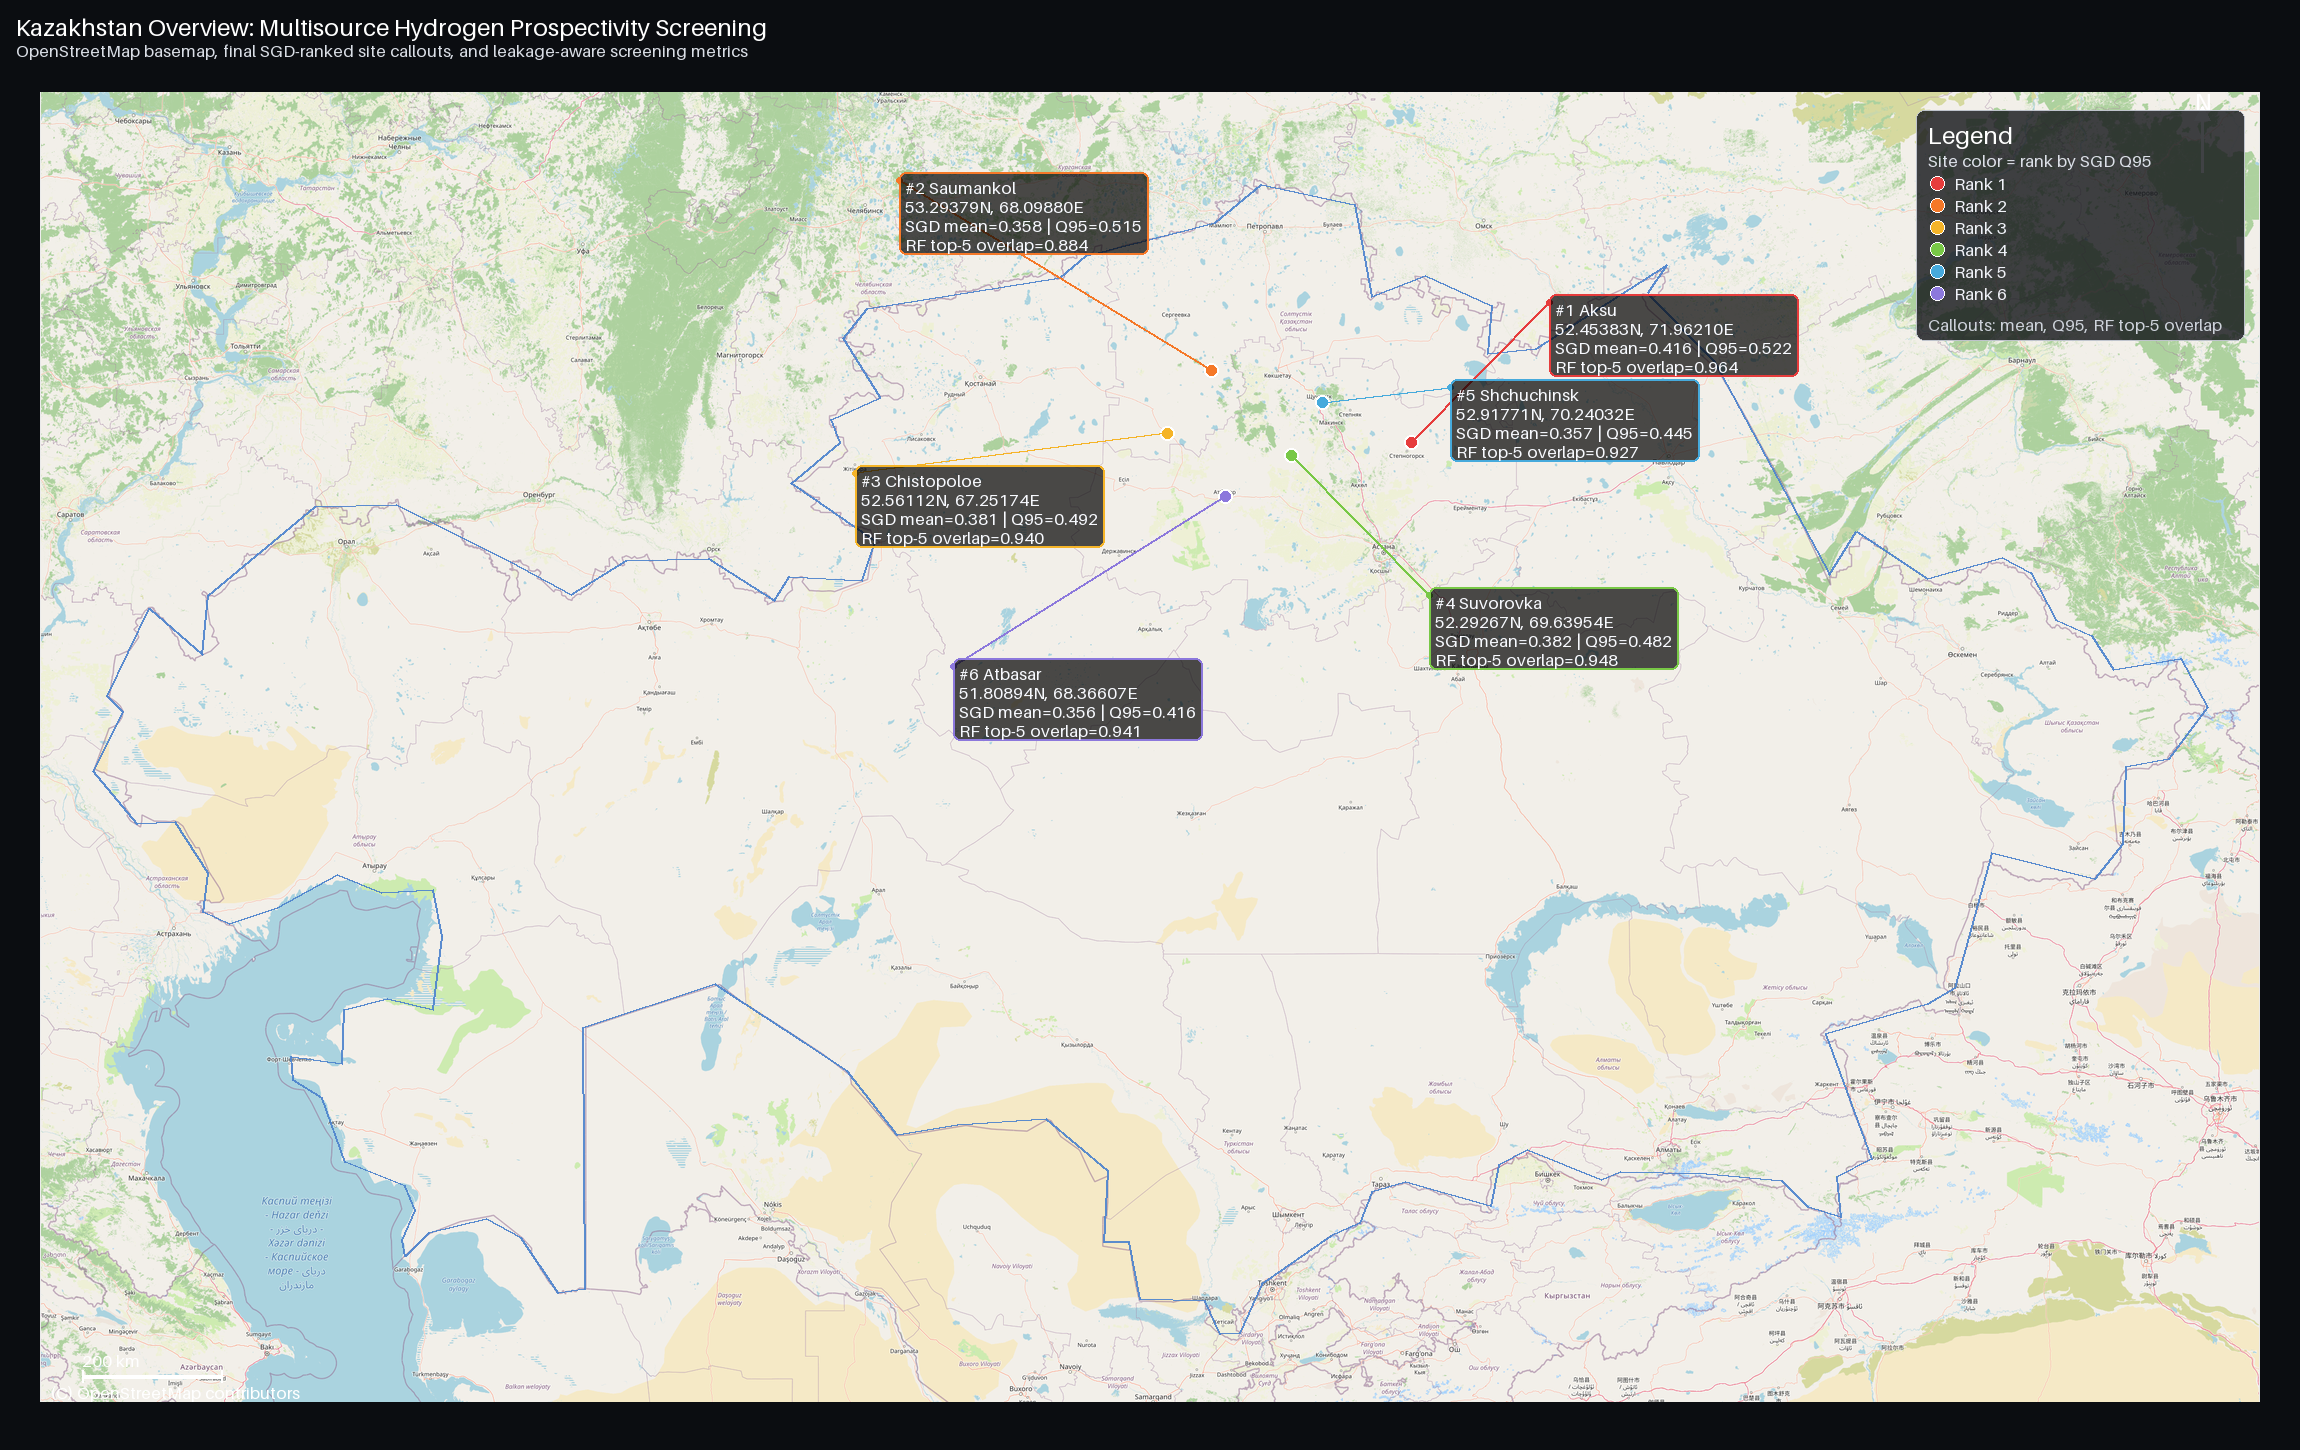
\includegraphics[width=\textwidth]{figures/00_overview/fig00_study_area.png}
\caption{Kazakhstan overview of the six reported natural-hydrogen anomaly sites. Colored callouts rank sites by final proxy-AOI SGD Q95 prospectivity and list coordinates, mean SGD score, Q95 score, and RF top-5\% overlap.}
\label{fig:study-area}
\end{figure}

Figure~\ref{fig:study-area} shows the practical consequence of this framing. The six sites are close enough that regional physiography may be shared, but far enough apart that a model must survive real spatial heterogeneity. The validation design therefore treats each site as a spatial block rather than as an interchangeable collection of pixels. Figure~\ref{fig:method-architecture} summarizes how that design constraint propagates through the full workflow, from observed evidence to final screening products.

\begin{figure}[!h]
\centering
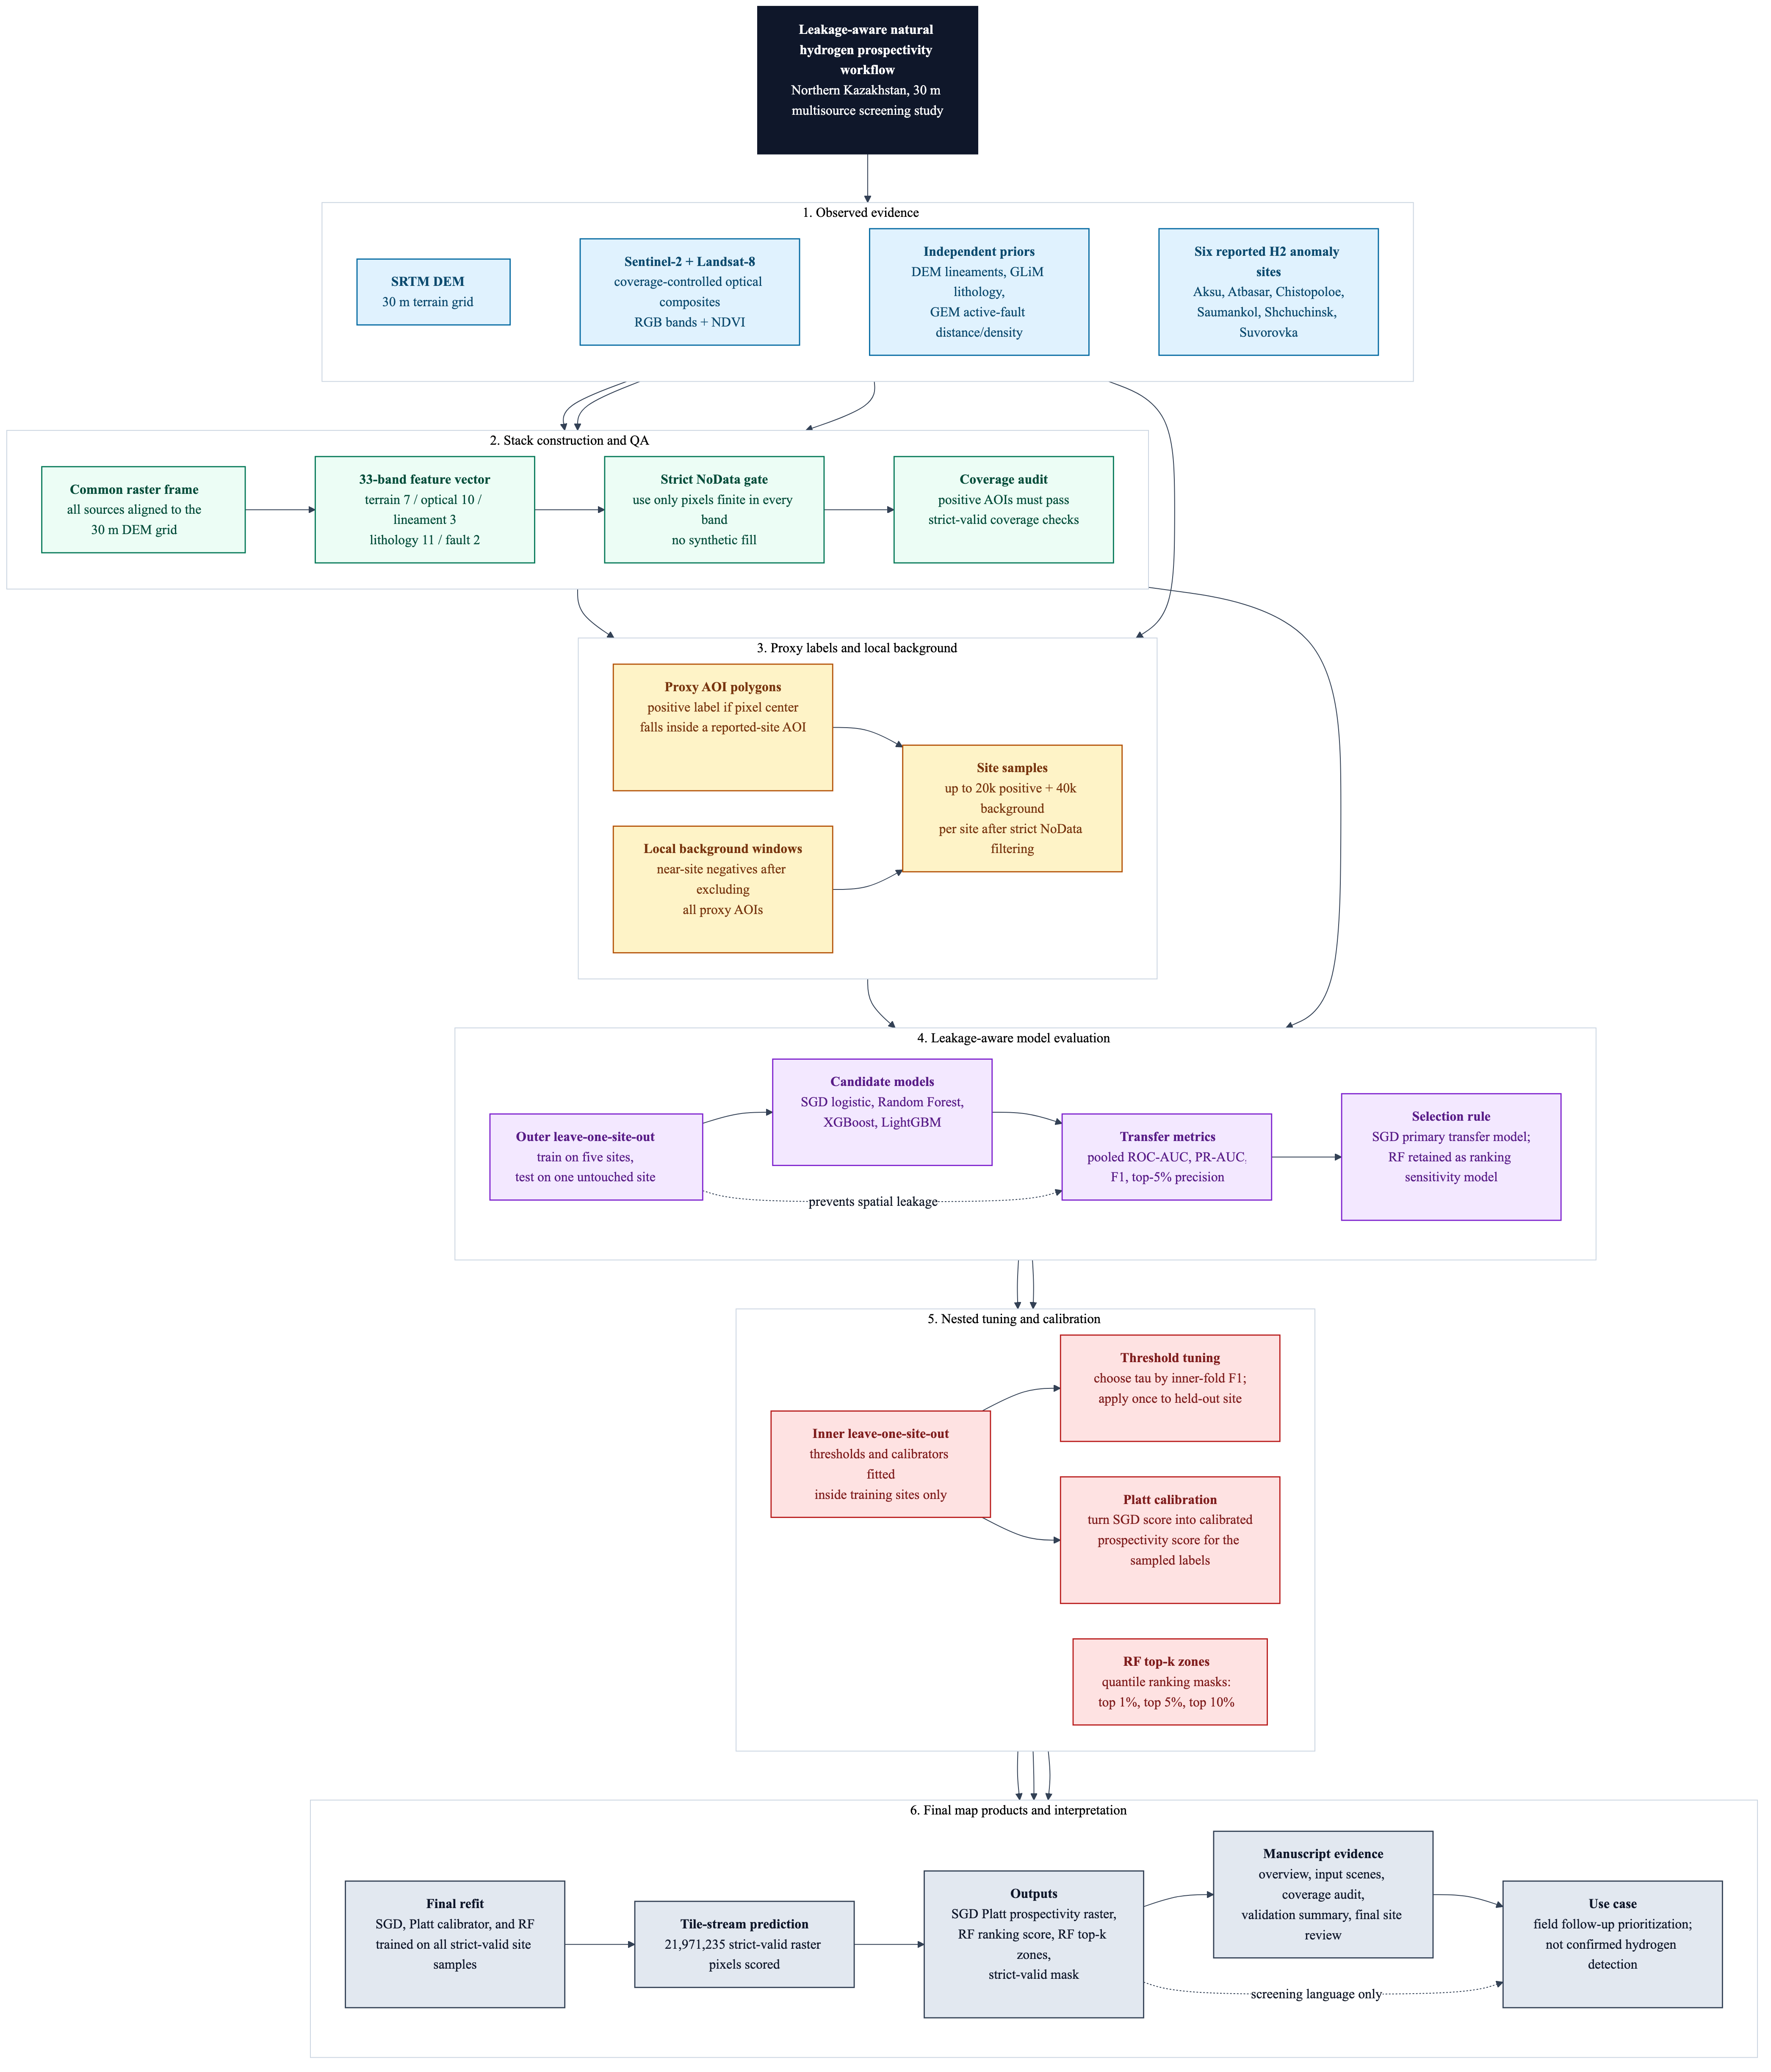
\includegraphics[width=\textwidth]{figures/00_overview/fig00_methodology_architecture.png}
\caption{Leakage-aware workflow from observed evidence to final screening products. Strict NoData retention and leave-one-site-out validation define the credibility controls for prospectivity and ranking-sensitivity outputs.}
\label{fig:method-architecture}
\end{figure}

\subsection{Input data and feature stack}
All raster predictors were aligned to the 30 m SRTM grid used for the study area \cite{farr2007srtm}. The final external-prior stack contains 33 bands. The first group contains terrain predictors derived from the DEM: elevation, slope, aspect, curvature, local relief, topographic position index, and roughness. These variables provide structural and geomorphic context, and they also give the model a stable baseline in areas where spectral imagery is incomplete.

The second group contains coverage-controlled Sentinel-2 and Landsat-8 optical predictors \cite{drusch2012sentinel,roy2014landsat8}. Four bands were retained from each sensor, together with Sentinel-2 NDVI and Landsat-8 NDVI. Earlier versions of the workflow exposed a serious coverage problem: some proxy-positive AOIs had little or no valid spectral coverage. We therefore rebuilt the Sentinel/Landsat source stacks using multi-scene, site-buffered coverage control and kept missing pixels as NoData. This was done because synthetic fill would have made the raster easier to model but harder to defend. It would blur the line between observed evidence and an invented surface.

The third group contains priors. DEM lineament strength, lineament density, and distance-to-lineament bands were included as leakage-safe structural features. Independent lithology was added from GLiM, producing 11 lithology classes inside the study area after clipping and filtering \cite{hartmann2012glim}. GEM Global Active Faults were also queried \cite{styron2020gem}; no active-fault traces intersected the 75 km buffered AOI, so the resulting fault layers are no-signal layers in this run. That absence is retained because it is part of the provenance of the independent prior stack, but it is interpreted cautiously as either a source limitation or a regional tectonic clue, not proof that faults are absent.

The assembled evidence layers are summarized visually as site-scale scene grids in Figures~\ref{fig:input-dem}, \ref{fig:input-sentinel}, \ref{fig:input-landsat}, \ref{fig:input-lineament}, and \ref{fig:input-lithology}, and as feature groups in Table~\ref{tab:feature-sources}. Each figure uses the same six zoom windows, clipped to the available model raster extent where a site touches the AOI edge, so that readers can compare the observed inputs site by site rather than reading another location map. The point of combining these sources is not that any single layer detects hydrogen. Rather, the stack asks whether terrain expression, seasonal optical response, mapped lithology, and structural priors jointly produce a repeatable ranking around reported anomaly sites.

\begin{figure}[!h]
\centering
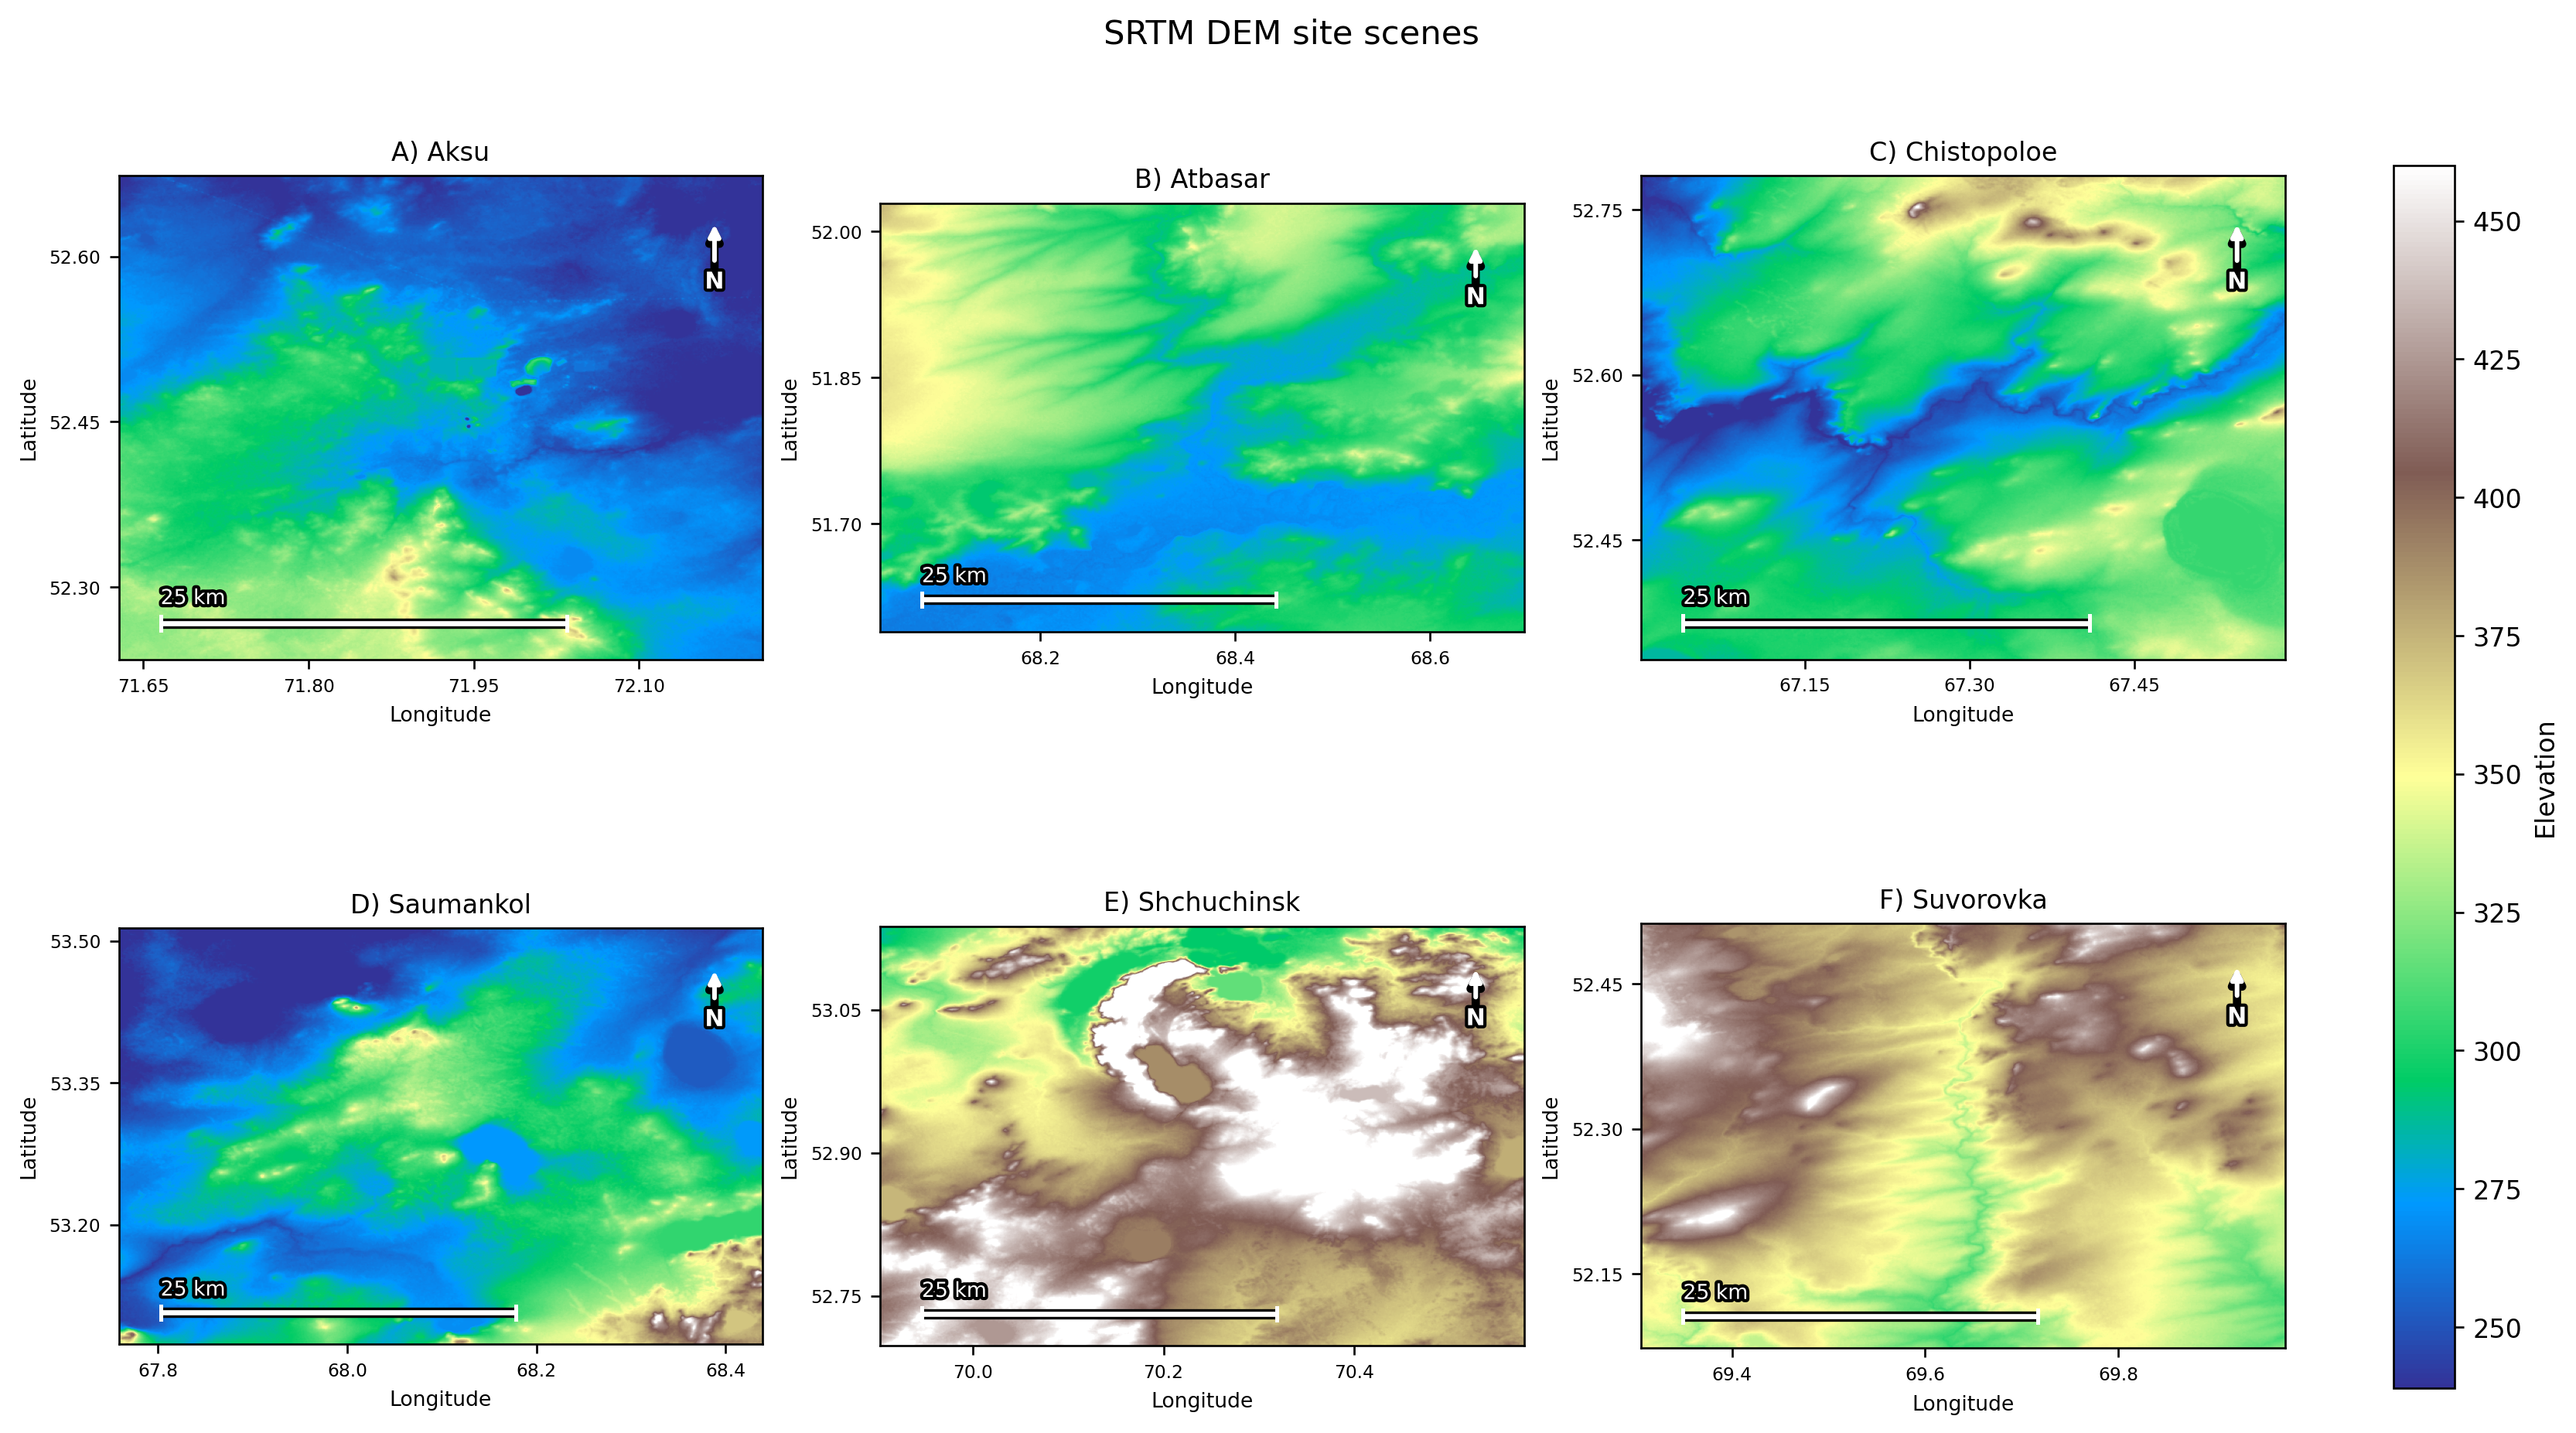
\includegraphics[width=\textwidth]{figures/01_inputs/01_input_stack_dem.png}
\caption{SRTM DEM site scenes for the six AOIs. Each panel uses the site-scale review window and includes longitude/latitude ticks, north arrow, and scale bar.}
\label{fig:input-dem}
\end{figure}

\begin{figure}[!h]
\centering
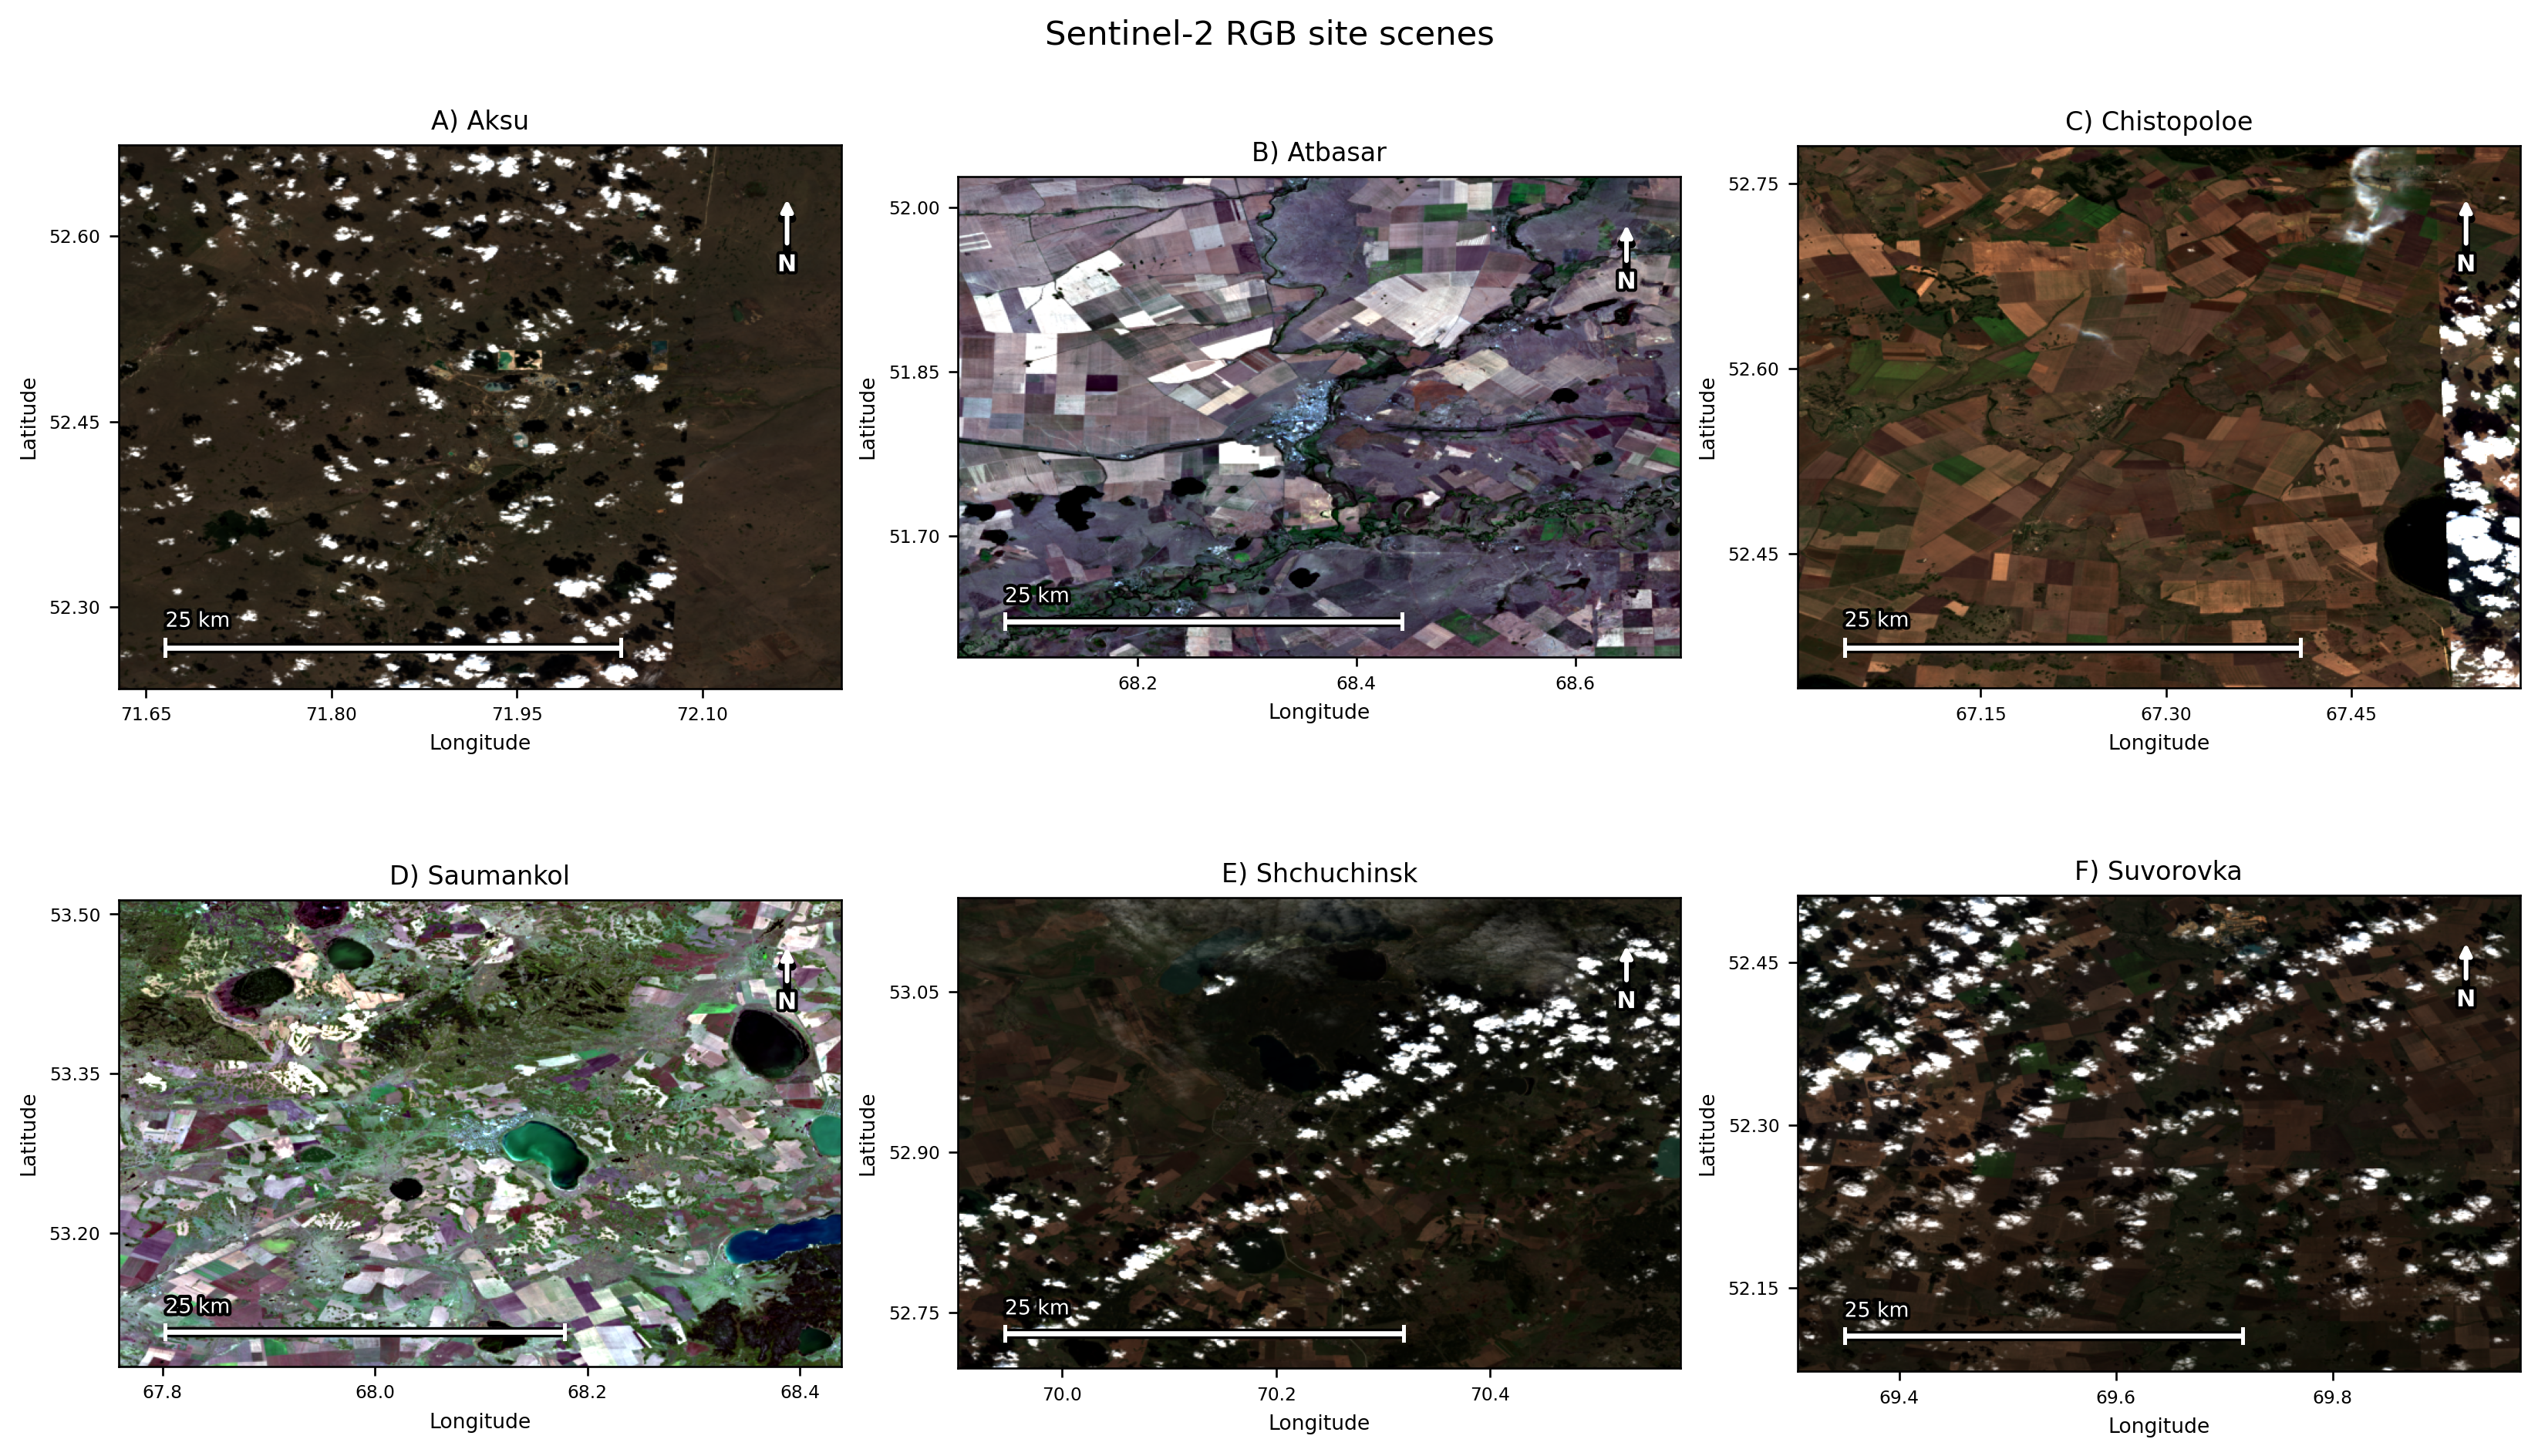
\includegraphics[width=\textwidth]{figures/01_inputs/01_input_stack_sentinel2_rgb.png}
\caption{Coverage-controlled Sentinel-2 RGB site scenes. The gray background marks pixels outside valid Sentinel-2 coverage after strict NoData handling.}
\label{fig:input-sentinel}
\end{figure}

\begin{figure}[!h]
\centering
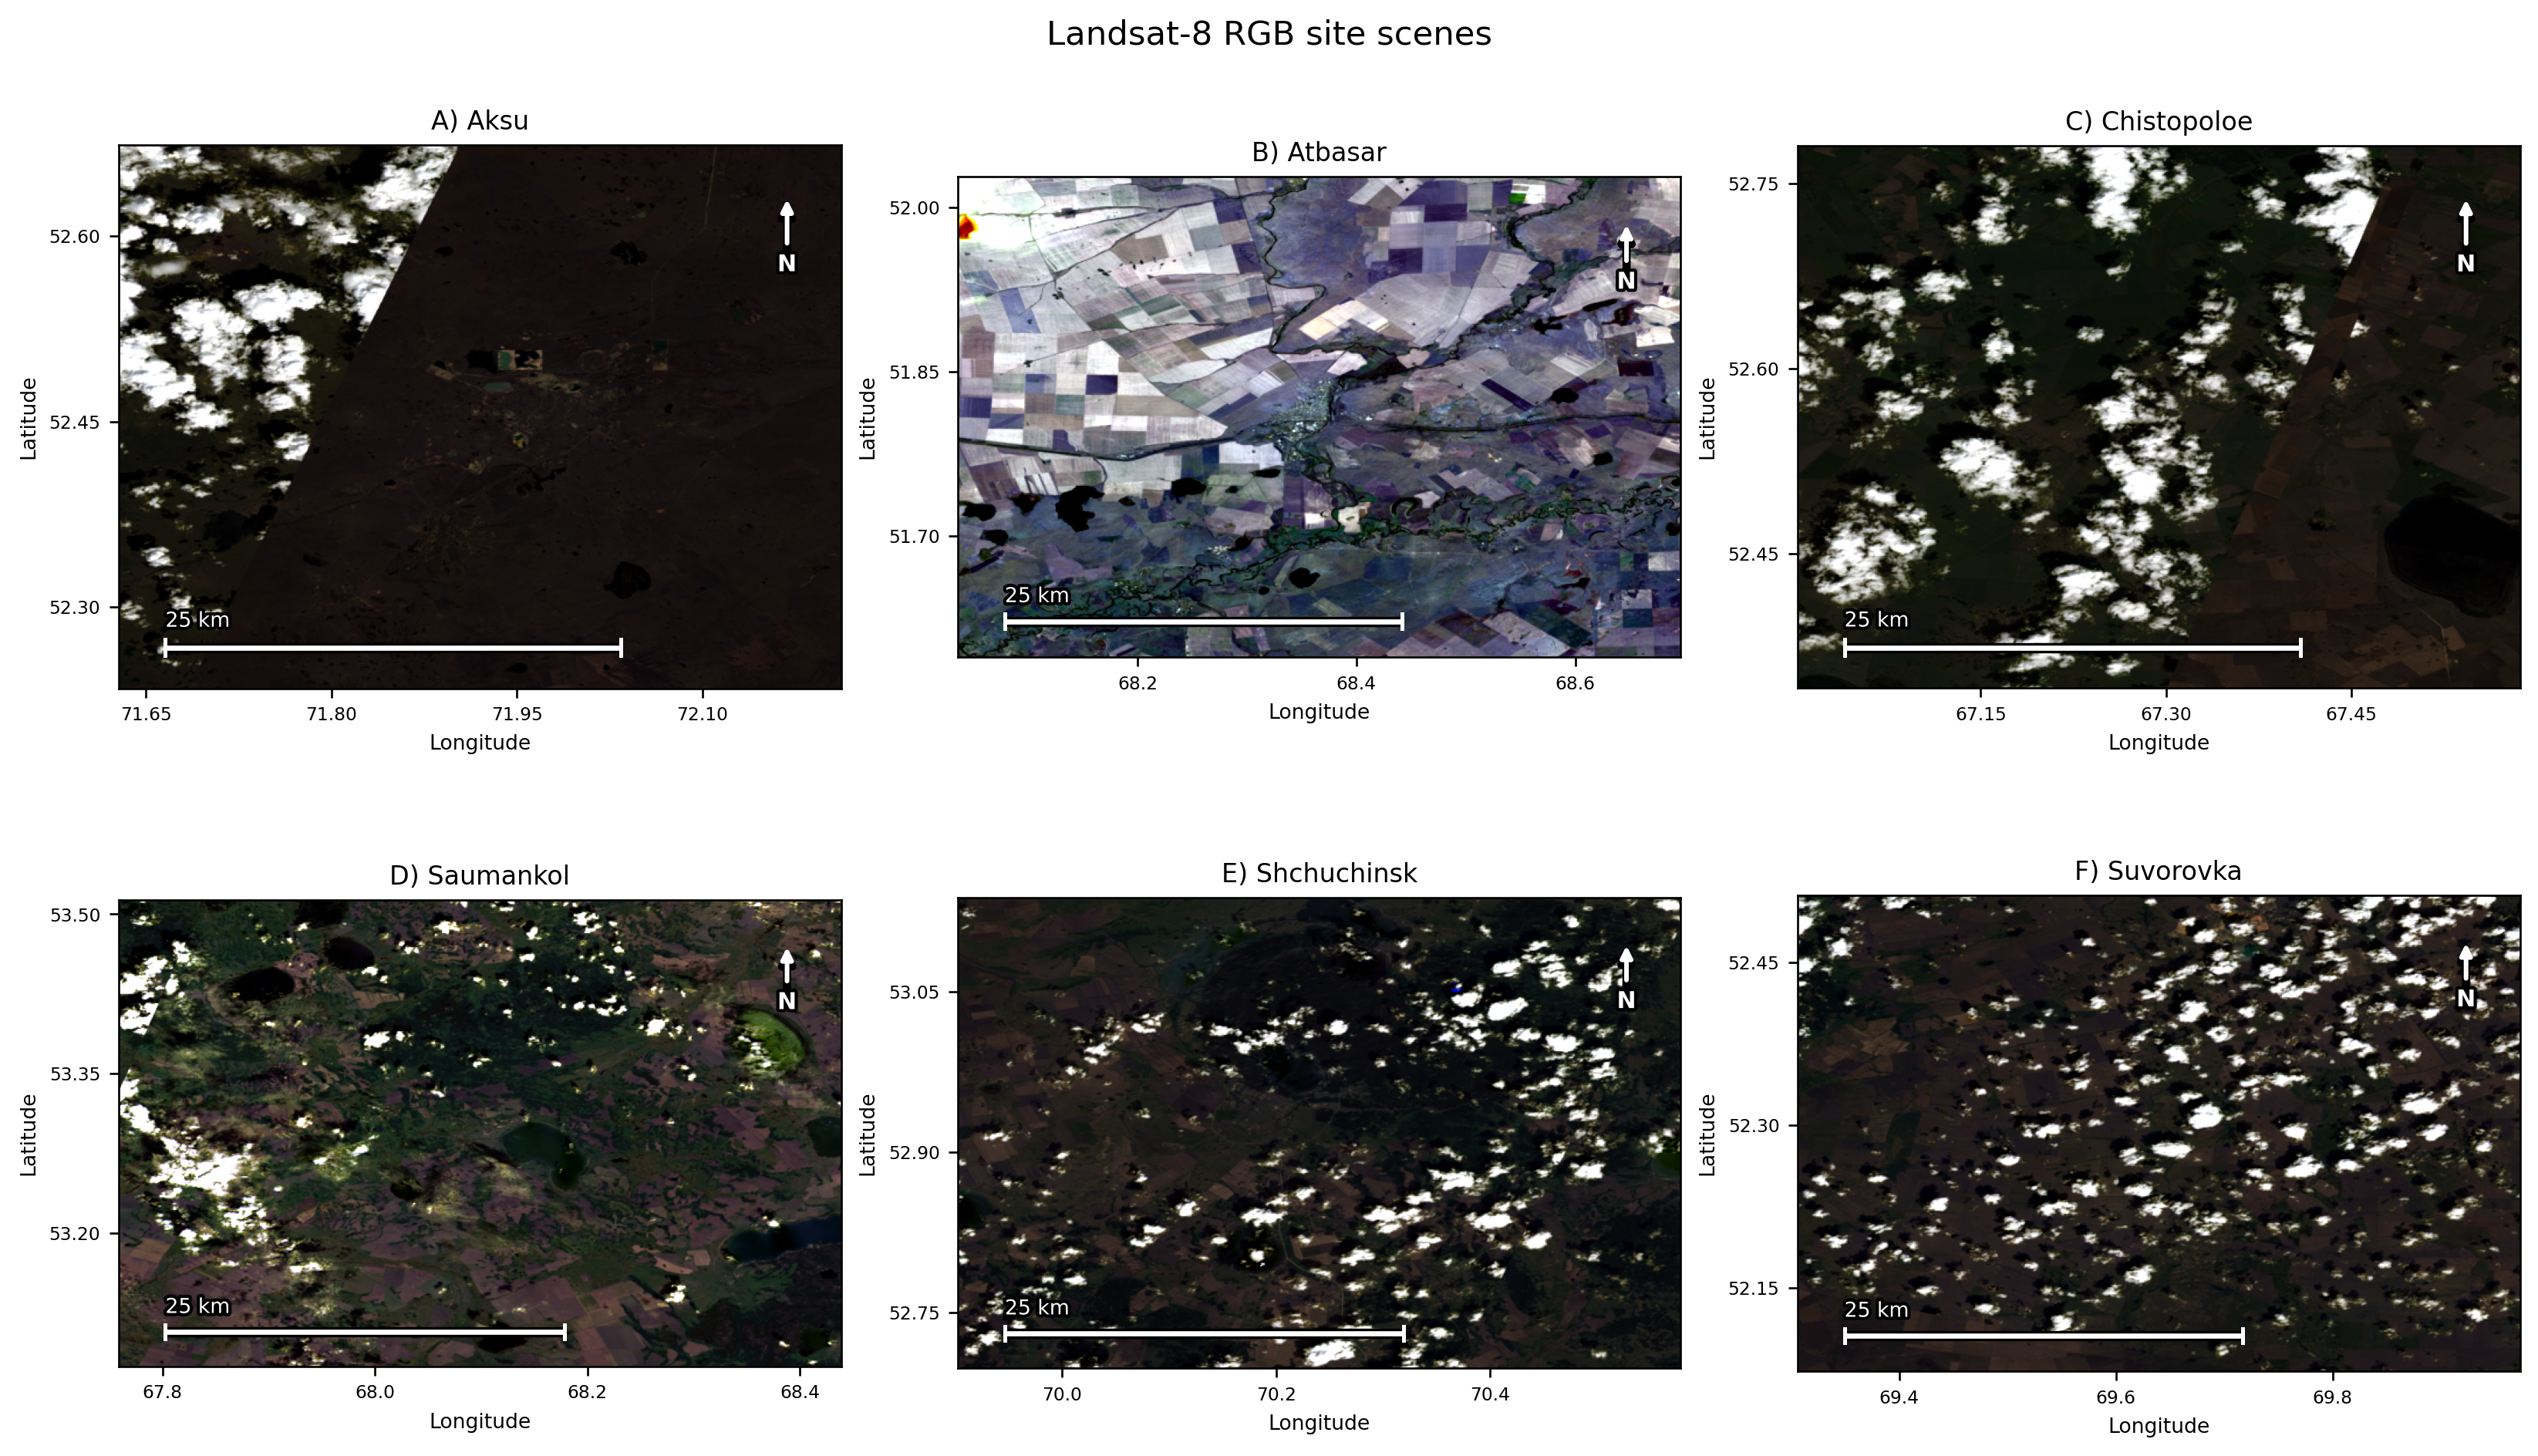
\includegraphics[width=\textwidth]{figures/01_inputs/01_input_stack_landsat8_rgb.png}
\caption{Coverage-controlled Landsat-8 RGB site scenes. The panels use the same site windows as Sentinel-2 for direct comparison of optical coverage and surface texture.}
\label{fig:input-landsat}
\end{figure}

\begin{figure}[!h]
\centering
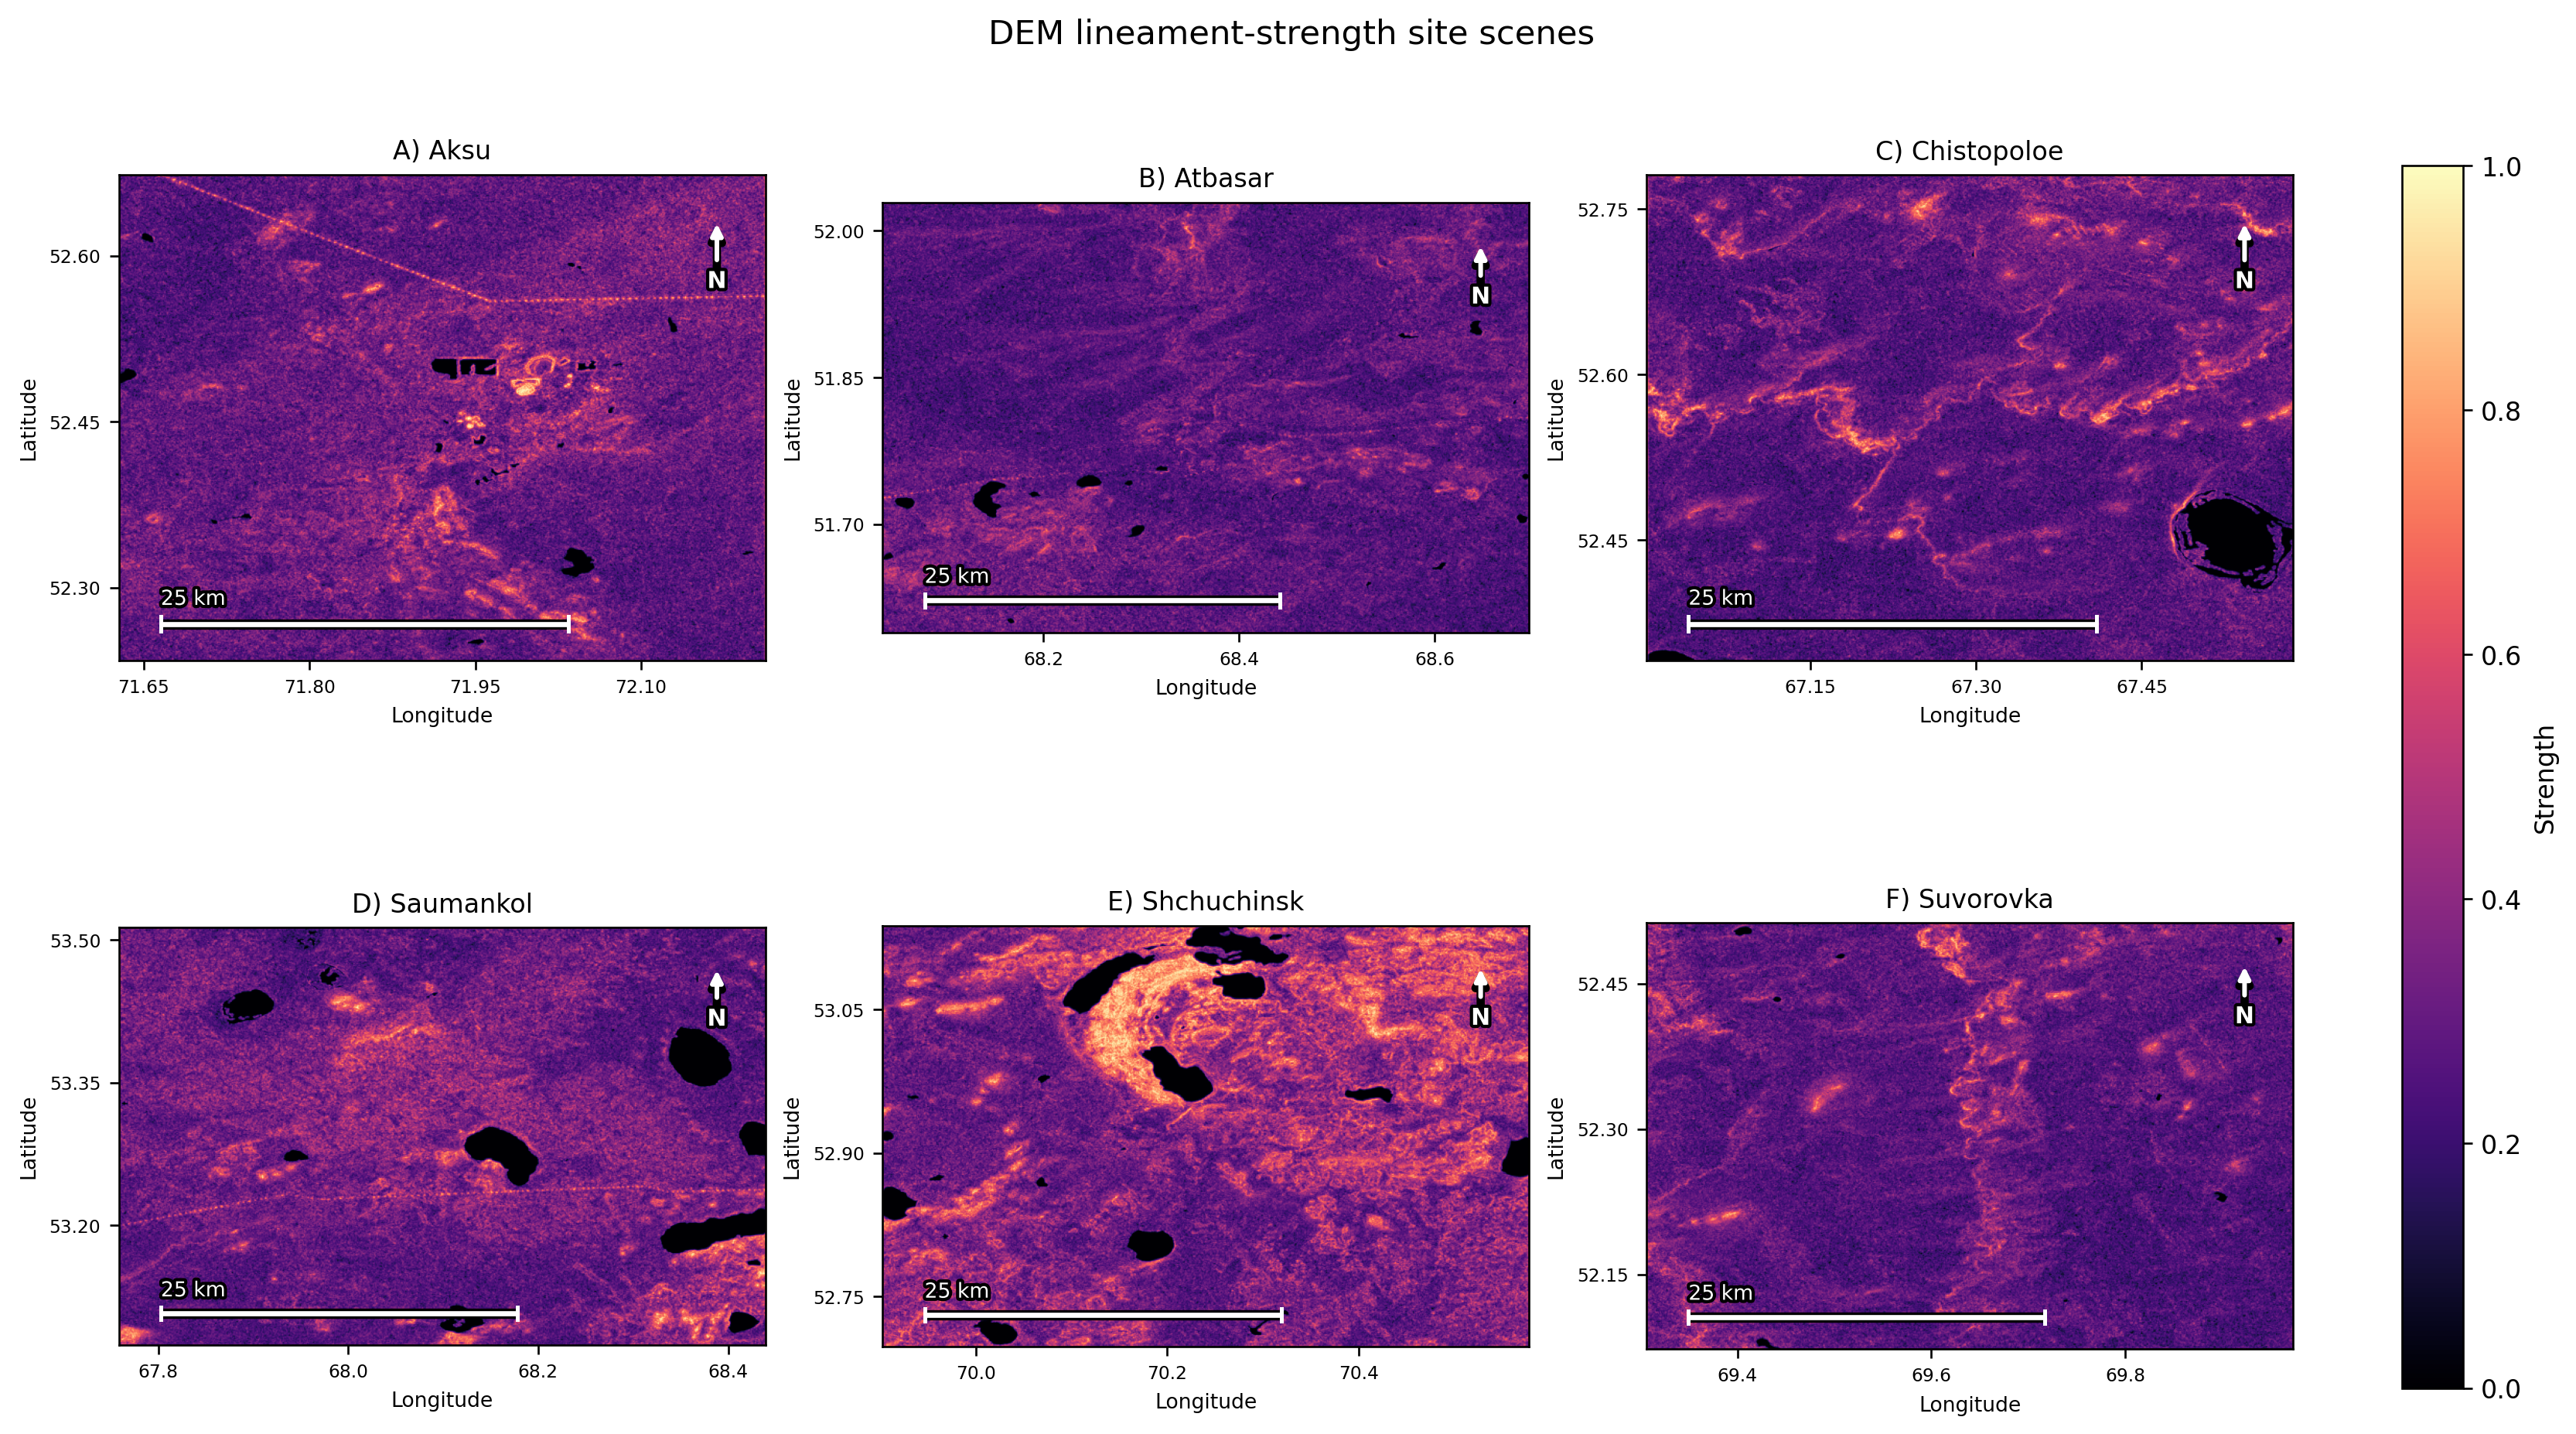
\includegraphics[width=\textwidth]{figures/01_inputs/01_input_stack_dem_lineament_strength.png}
\caption{DEM-derived lineament-strength site scenes. The priors express terrain morphology as leakage-safe structural context, not field-confirmed mapped faults.}
\label{fig:input-lineament}
\end{figure}

\begin{figure}[!h]
\centering
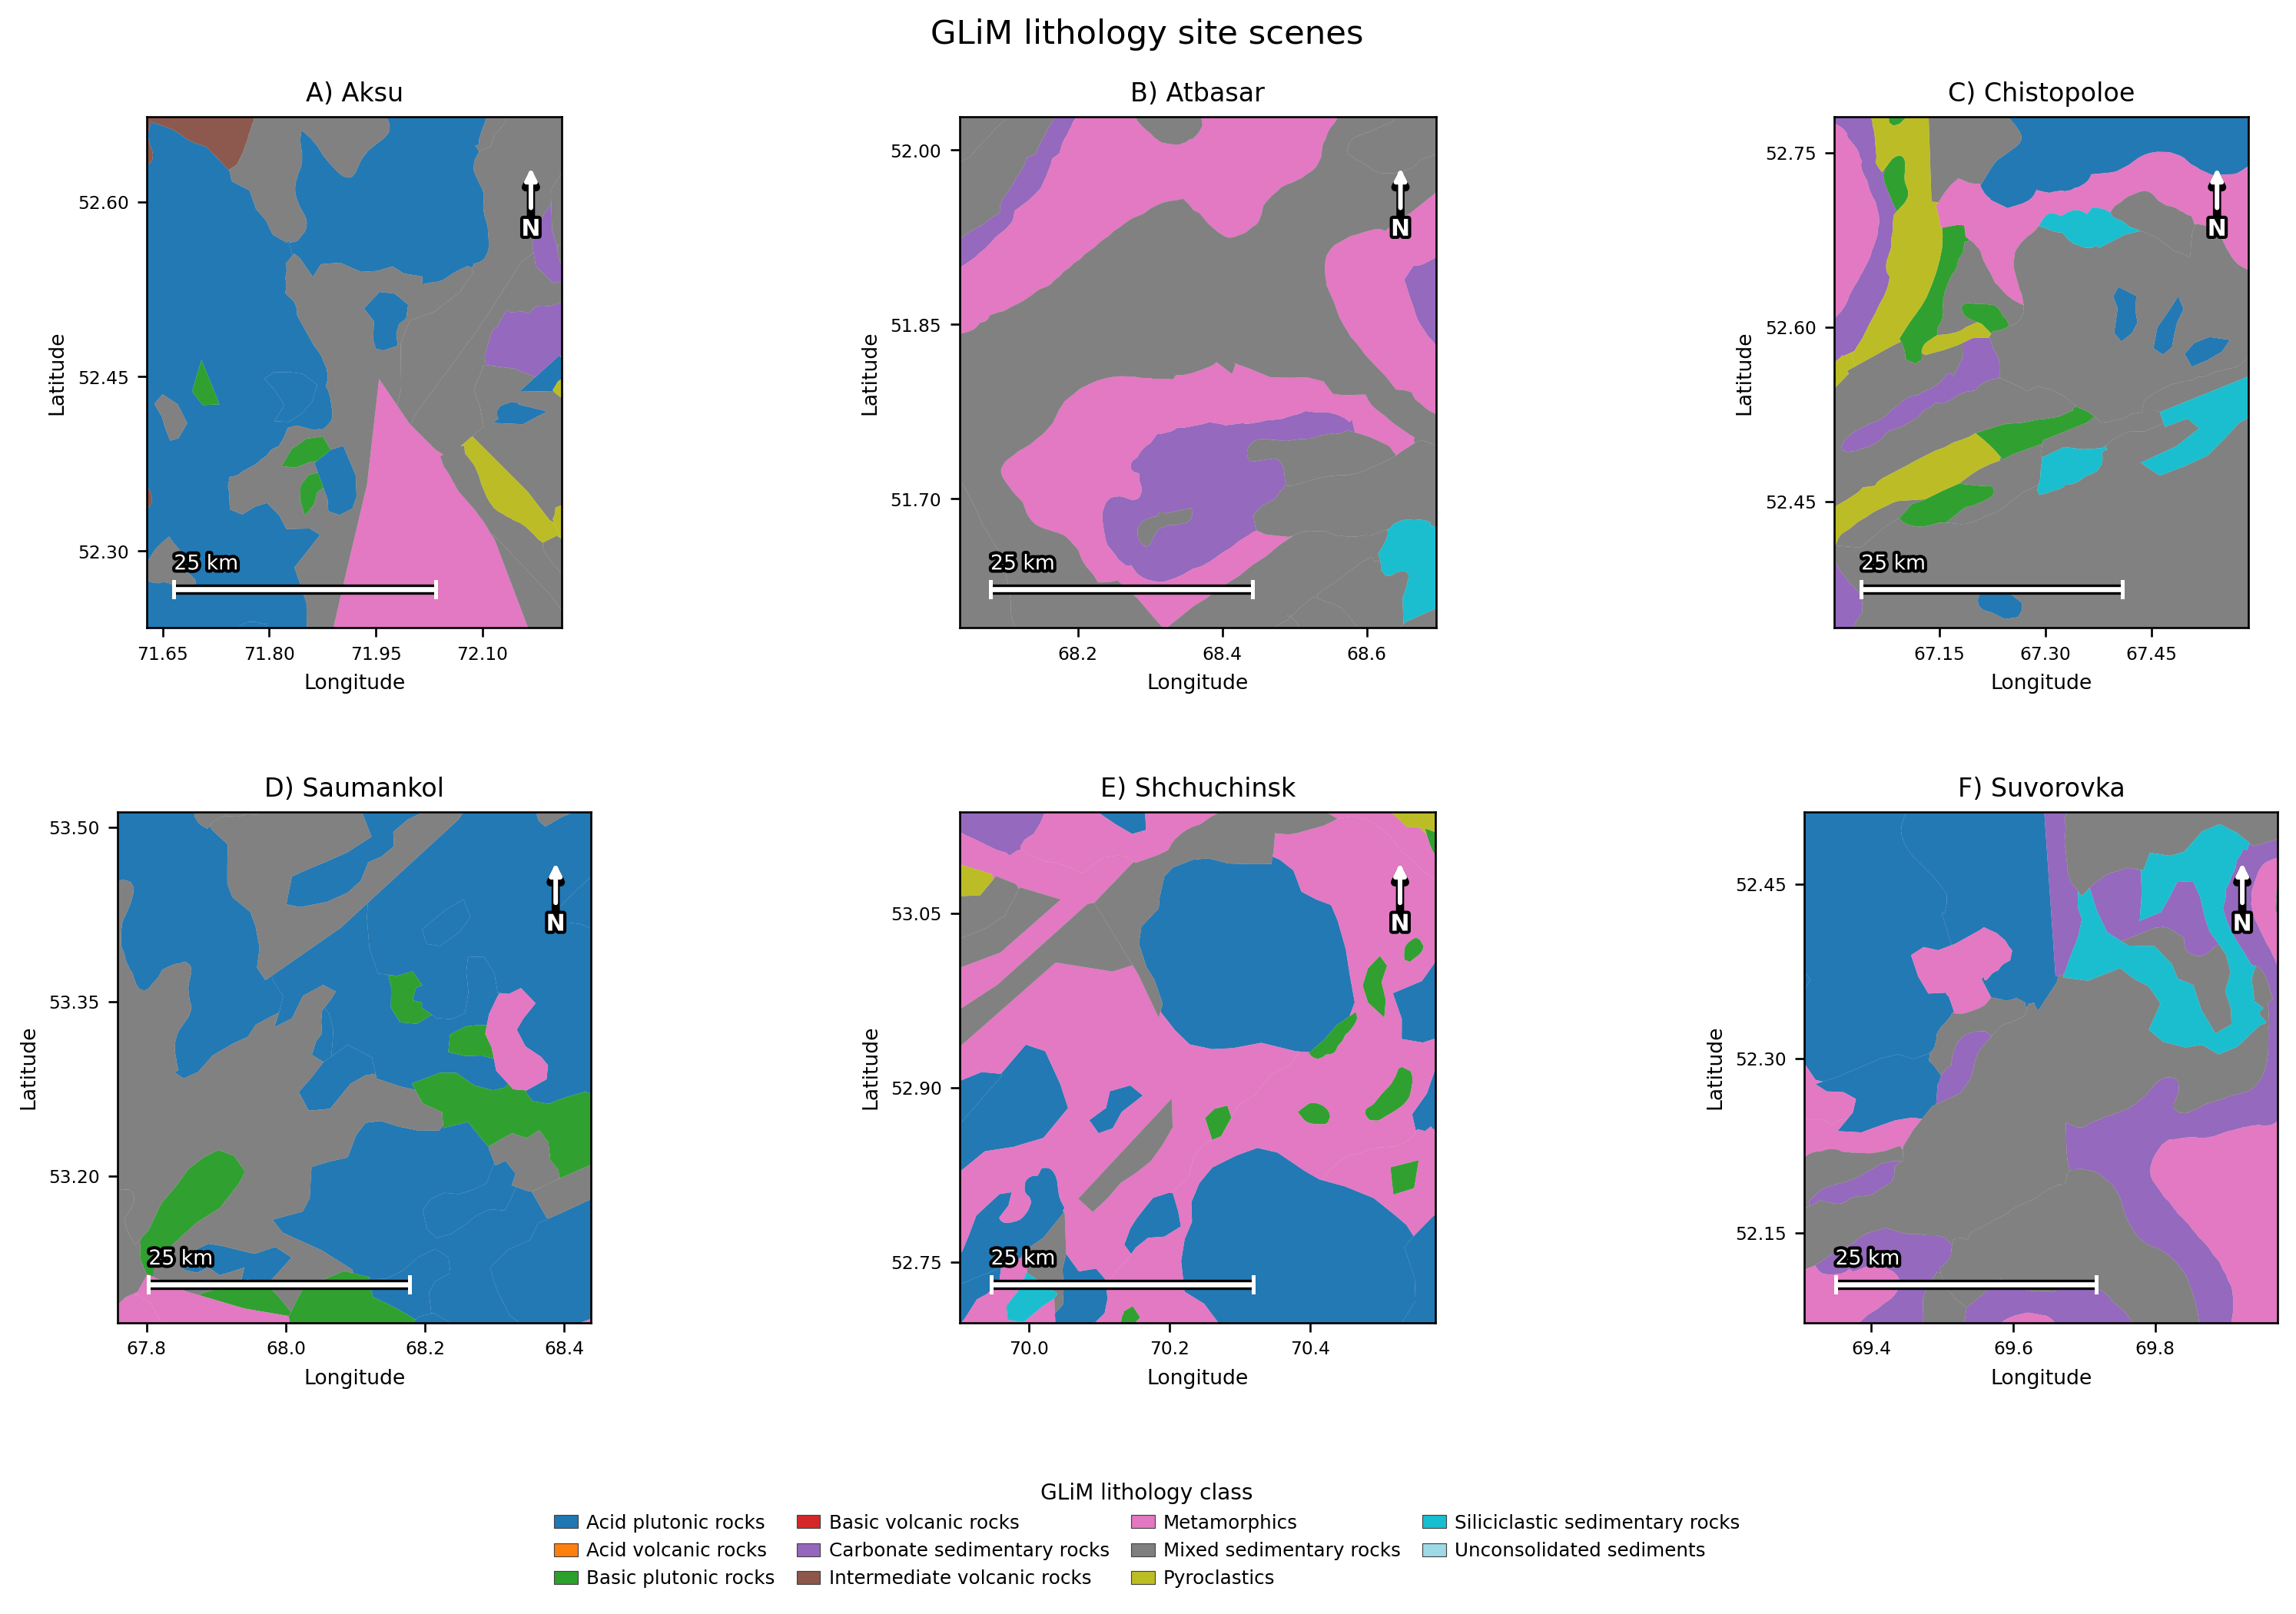
\includegraphics[width=\textwidth]{figures/01_inputs/01_input_stack_glim_lithology.png}
\caption{GLiM lithology site scenes with class legend. The panels show independent regional geological context in the six site-scale review windows.}
\label{fig:input-lithology}
\end{figure}

\begin{table}[t]
\centering
\caption{Feature groups in the final external-prior stack. Each group provides screening context rather than direct evidence of hydrogen occurrence.}
\label{tab:feature-sources}
\begin{tabular}{p{0.20\textwidth}p{0.28\textwidth}rp{0.34\textwidth}}
\toprule
Group & Source & Bands & Role in the screening model \\
\midrule
DEM terrain & SRTM derivatives \cite{farr2007srtm} & 7 & Structural and geomorphic baseline for all sites \\
Optical spectra & Sentinel-2 and Landsat-8 composites \cite{drusch2012sentinel,roy2014landsat8} & 10 & Surface spectral and vegetation context where observed coverage is valid \\
DEM lineament priors & DEM-derived structural proxies & 3 & Leakage-safe lineament strength, density, and distance context \\
Lithology & GLiM regional lithology \cite{hartmann2012glim} & 11 & Independent regional geology classes clipped to the AOI \\
Active faults & GEM Global Active Faults \cite{styron2020gem} & 2 & Fault distance and density layers; no mapped active-fault traces intersected the buffered AOI \\
Total & Multisource 30 m stack & 33 & Final pixel vector used for model comparison and map generation \\
\bottomrule
\end{tabular}
\end{table}

Let \(i\) index pixels and \(j=1,\ldots,p\) index feature bands. The final pixel vector is
\begin{equation}
    \mathbf{x}_i =
    \left[
    \mathbf{x}^{\mathrm{DEM}}_i,
    \mathbf{x}^{\mathrm{S2}}_i,
    \mathbf{x}^{\mathrm{L8}}_i,
    \mathbf{x}^{\mathrm{prior}}_i
    \right] \in \mathrm{R}^{p},
    \qquad p=33 .
    \label{eq:feature-vector}
\end{equation}
Strict-valid pixels are those for which every band is finite and no band equals its raster NoData code \(\eta_j\):
\begin{equation}
    m_i =
    \mathbf{1}
    \left\{
    \bigwedge_{j=1}^{p}
    \left(
    \operatorname{finite}(x_{ij})
    \land
    x_{ij} \ne \eta_j
    \right)
    \right\}.
    \label{eq:strict-valid}
\end{equation}
Only pixels with \(m_i=1\) are used for training, validation, and final prediction. This single rule is important: it prevents the model from learning that a NoData code such as \(-9999\) is a geological signal.

\subsection{Proxy labels and local background}
Let \(A_k\) denote the proxy anomaly polygon for site \(k\), with \(k=1,\ldots,6\). A pixel is assigned a positive proxy label when its center falls inside one of these polygons:
\begin{equation}
    y_i =
    \mathbf{1}
    \left\{
    s_i \in \bigcup_{k=1}^{6} A_k
    \right\},
    \label{eq:proxy-label}
\end{equation}
where \(s_i\) is the pixel location. Negative samples are drawn from local background windows around each site after excluding the held-out site's proxy polygon and the other proxy polygons. This design makes the negative class more demanding than a random landscape background, because the model must distinguish the reported site vicinity from nearby non-proxy pixels. It also keeps the task aligned with exploration practice: a field team does not need a continent-scale binary answer first; it needs to know which local zones deserve follow-up.

For the final site-blocked experiments, each site contributed up to 20,000 positive pixels and 40,000 local-background pixels after strict NoData exclusion. Across six sites, the final sampled training population contained 360,000 pixels with a controlled positive rate of 0.3333.

\subsection{Model families and selection rule}
Four model families were compared on the final external-prior stack: a regularized SGD logistic classifier implemented through scikit-learn, random forest, XGBoost, and LightGBM \cite{pedregosa2011scikit,breiman2001randomforests,chen2016xgboost,ke2017lightgbm}. The tree models were included because they can capture nonlinear interactions between terrain, spectral, and lithologic variables. The linear SGD model was included for the opposite reason: if spatial transfer is fragile, a simpler regularized model can be more trustworthy than a model with enough capacity to memorize site-specific texture.

The SGD model estimates a susceptibility score through a logistic link:
\begin{equation}
    \hat{p}_i =
    \sigma
    \left(
    \beta_0 + \mathbf{x}_i^{\top}\boldsymbol{\beta}
    \right),
    \qquad
    \sigma(u)=\frac{1}{1+\exp(-u)}.
    \label{eq:sgd-logit}
\end{equation}
With class weights \(w_i\), the regularized objective is
\begin{equation}
    \underset{\beta_0,\boldsymbol{\beta}}{\arg\min}
    \sum_i
    w_i
    \left[
    -y_i\log(\hat{p}_i)
    -(1-y_i)\log(1-\hat{p}_i)
    \right]
    +
    \alpha \lVert \boldsymbol{\beta} \rVert_2^2 .
    \label{eq:sgd-objective}
\end{equation}
Focused tuning tested \(\alpha\in\{10^{-5},3\times10^{-5},10^{-4},3\times10^{-4},10^{-3}\}\). The best site-blocked setting was \(\alpha=10^{-4}\), which was then carried forward as the primary model.

\subsection{Site-blocked validation, threshold tuning, and calibration}
For leave-one-site-out validation, the training and test sets for outer fold \(k\) are
\begin{equation}
    \mathcal{D}^{(k)}_{\mathrm{train}}
    =
    \bigcup_{\ell\ne k}\mathcal{D}_{\ell},
    \qquad
    \mathcal{D}^{(k)}_{\mathrm{test}}
    =
    \mathcal{D}_{k}.
    \label{eq:loso}
\end{equation}
This is the central leakage control in the study. It deliberately makes the test harder: if Chistopoloe is held out, no Chistopoloe proxy or local background pixels are used to fit the model. The same logic motivates spatial blocking in other spatial prediction settings where naive random folds can produce optimistic transfer estimates \cite{roberts2017crossvalidation,valavi2019blockcv}.

Thresholded metrics were not selected using the held-out test site. Instead, each outer fold used an inner leave-one-site-out loop over the training sites. The selected threshold for outer fold \(k\) is
\begin{equation}
    \tau_k^\star =
    \underset{\tau\in\mathcal{T}}{\arg\max}
    \;
    F_1
    \left(
    \mathcal{D}^{(k)}_{\mathrm{inner}},
    \tau
    \right),
    \qquad
    \mathcal{T}=\{0.01,0.02,\ldots,0.99\}.
    \label{eq:threshold}
\end{equation}
The chosen \(\tau_k^\star\) is then applied once to the outer held-out site. This nested design matters because a threshold can overfit just as easily as a model can. Precision-recall diagnostics are emphasized because the positive proxy class is sparse relative to the landscape, a setting where PR curves are often more informative than ROC curves alone \cite{saito2015precision}.

Probability calibration was handled with the same leakage-aware logic. For each outer fold, inner out-of-fold predictions from the training sites were used to fit Platt and isotonic calibrators \cite{platt1999probabilistic}. The Platt transformation is
\begin{equation}
    \tilde{p}_i =
    \sigma
    \left(
    a\hat{p}_i + b
    \right),
    \label{eq:platt}
\end{equation}
where \(a\) and \(b\) are fitted only from training-site out-of-fold predictions. The calibrated value \(\tilde{p}_i\) is described as a calibrated prospectivity score for the sampled proxy-label distribution. It is not described as a field-confirmed probability of hydrogen occurrence.

The random forest model is retained as a ranking sensitivity model. For a top fraction \(\gamma\), the RF sensitivity zone is defined as
\begin{equation}
    Z_{\gamma}
    =
    \{i:r_i\ge Q_{1-\gamma}(r)\},
    \label{eq:topk}
\end{equation}
where \(r_i\) is the RF score and \(Q_{1-\gamma}(r)\) is the empirical \((1-\gamma)\)-quantile over strict-valid pixels. These zones answer a practical ranking question: where do the most aggressive nonlinear rankings concentrate?

\begin{algorithm}[H]
\caption{Leakage-aware prospectivity workflow}
\label{alg:workflow}
\begin{algorithmic}[1]
\Require DEM, Sentinel-2, Landsat-8, GLiM lithology, GEM faults, proxy site polygons
\Ensure Calibrated SGD prospectivity raster, RF top-k sensitivity zones, validation reports
\State Align all raster sources to the 30 m DEM grid
\State Derive DEM terrain features, spectral indices, lineament priors, lithology bands, and fault bands
\State Build strict-valid mask using Equation~\ref{eq:strict-valid}
\For{each site \(k\in\{1,\ldots,6\}\)}
    \State Rasterize proxy anomaly polygon \(A_k\)
    \State Sample positive pixels inside \(A_k\)
    \State Sample local background pixels in the buffered site block
\EndFor
\For{each candidate model family}
    \For{each held-out site \(k\)}
        \State Train on \(\bigcup_{\ell\ne k}\mathcal{D}_{\ell}\)
        \State Predict on \(\mathcal{D}_{k}\)
        \State Store ROC-AUC, PR-AUC, F1, and top-k precision
    \EndFor
    \State Rank the model by pooled site-blocked PR-AUC
\EndFor
\State Select SGD as the primary spatial-transfer model
\State Retain RF as the top-k ranking sensitivity model
\For{each outer held-out site \(k\)}
    \For{each inner held-out training site \(h\ne k\)}
        \State Train on the remaining training sites
        \State Predict on site \(h\)
    \EndFor
    \State Select \(\tau_k^\star\) from inner predictions using Equation~\ref{eq:threshold}
    \State Fit Platt calibration from inner out-of-fold predictions using Equation~\ref{eq:platt}
    \State Evaluate threshold and calibration on the untouched outer site \(k\)
\EndFor
\State Fit final SGD, final Platt calibrator, and final RF using all strict-valid site samples
\State Stream the full raster by tiles and write final prospectivity and sensitivity maps
\end{algorithmic}
\end{algorithm}

\section{Results}
\subsection{Coverage control changed the interpretation before it changed the model}
The first important result was not a model score. It was the coverage audit. Earlier fusion runs appeared promising under random pixel splits, but strict NoData auditing showed that several proxy-positive AOIs lacked valid spectral observations. A high score from such a stack would be scientifically ambiguous because the model could learn the pattern of missingness rather than the pattern of prospectivity.

After the Sentinel-2 and Landsat-8 rebuild, all six positive AOIs passed the 0.95 strict-valid feature-group coverage gate (Figure~\ref{fig:coverage-audit}). The final map pass scored 21,971,235 strict-valid raster pixels. This changed the status of the experiment: the NoData blocker over positive AOIs was no longer the dominant limitation. The dominant limitation became spatial transfer across proxy sites.

\begin{figure}[t]
\centering
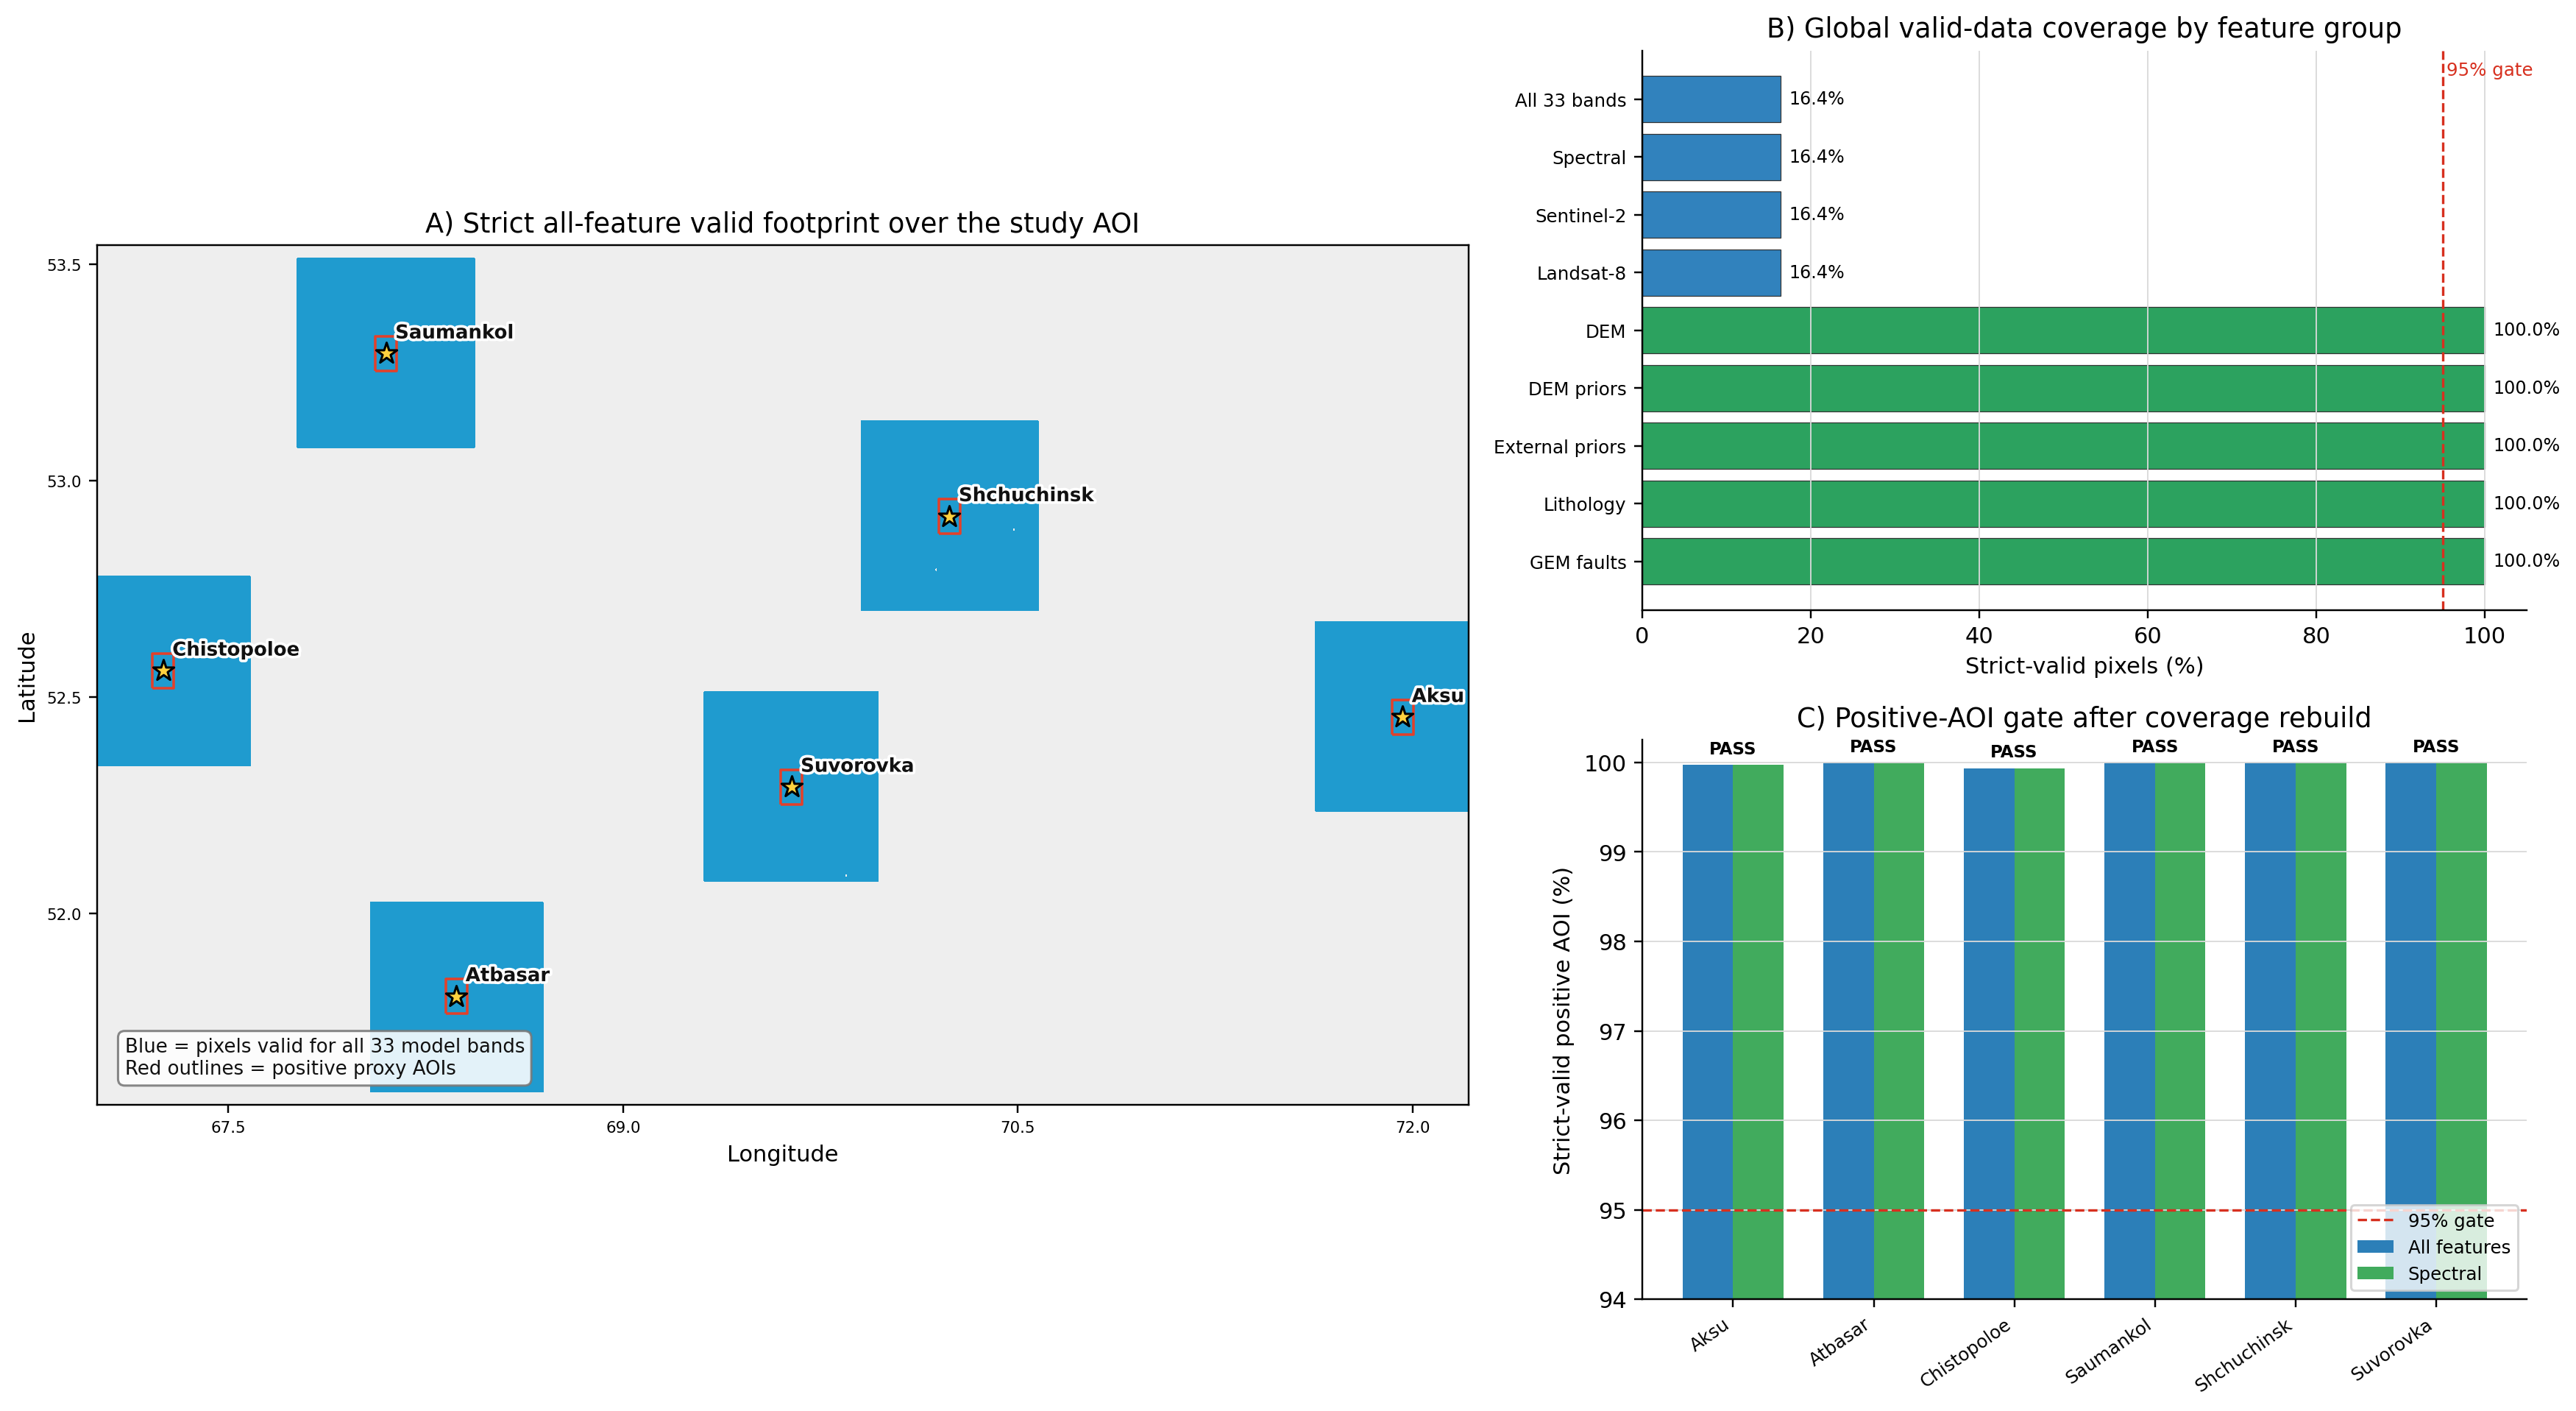
\includegraphics[width=\textwidth]{figures/02_feature_coverage/fig02_coverage_audit.png}
\caption{Strict valid-data audit for the final external-prior stack. Panel A maps the all-feature footprint, Panel B summarizes feature-group coverage, and Panel C confirms that every positive proxy AOI exceeds the 0.95 strict-valid gate.}
\label{fig:coverage-audit}
\end{figure}

\subsection{External priors helped, but did not erase site heterogeneity}
The external-prior stack added independent lithology context from GLiM and fault context from GEM. GLiM contributed 571 clipped lithology polygons and 11 modeled lithology classes. GEM active faults contributed no active-fault traces inside the buffered AOI, so the fault bands carried little to no signal in this run. This outcome is still useful because it prevents the model from inventing a fault relationship where the selected public source does not provide one.

Compared with the coverage-controlled XGBoost run, the external-prior XGBoost run modestly improved site-blocked PR-AUC from 0.3459 to 0.3687. The improvement is real enough to justify carrying the external-prior stack forward, but it is not large enough to claim that lithology solved the transfer problem. The interpretation is more measured: independent lithology adds regional geological context, while the proxy-label design and site heterogeneity still dominate the uncertainty.

\subsection{Model selection favored the simpler transfer model}
Table~\ref{tab:model-comparison} and Figure~\ref{fig:validation-summary} summarize the strict leave-one-site-out comparison on the final 33-band external-prior stack. The SGD model ranked first by pooled ROC-AUC and PR-AUC. This was not the expected outcome if one only looked at random splits, where RF, XGBoost, and LightGBM appeared much stronger. Under site-blocked testing, however, the higher-capacity models did not transfer as well.

\begin{table}[t]
\centering
\caption{Strict leave-one-site-out model comparison on the external-prior stack. The primary selection metric is pooled PR-AUC because the positive class is sparse and the task is ranking-oriented.}
\label{tab:model-comparison}
\begin{tabular}{lrrrrrr}
\toprule
Model & ROC-AUC & PR-AUC & Precision & Recall & F1 & Top-5\% precision \\
\midrule
SGD & 0.6173 & 0.4096 & 0.3984 & 0.0531 & 0.0937 & 0.4091 \\
Random forest & 0.5372 & 0.3990 & 0.5530 & 0.0101 & 0.0198 & 0.5995 \\
XGBoost & 0.4997 & 0.3687 & 0.4838 & 0.0908 & 0.1529 & 0.5008 \\
LightGBM & 0.5074 & 0.3654 & 0.4751 & 0.0711 & 0.1237 & 0.4751 \\
\bottomrule
\end{tabular}
\end{table}

\begin{figure}[!h]
\centering
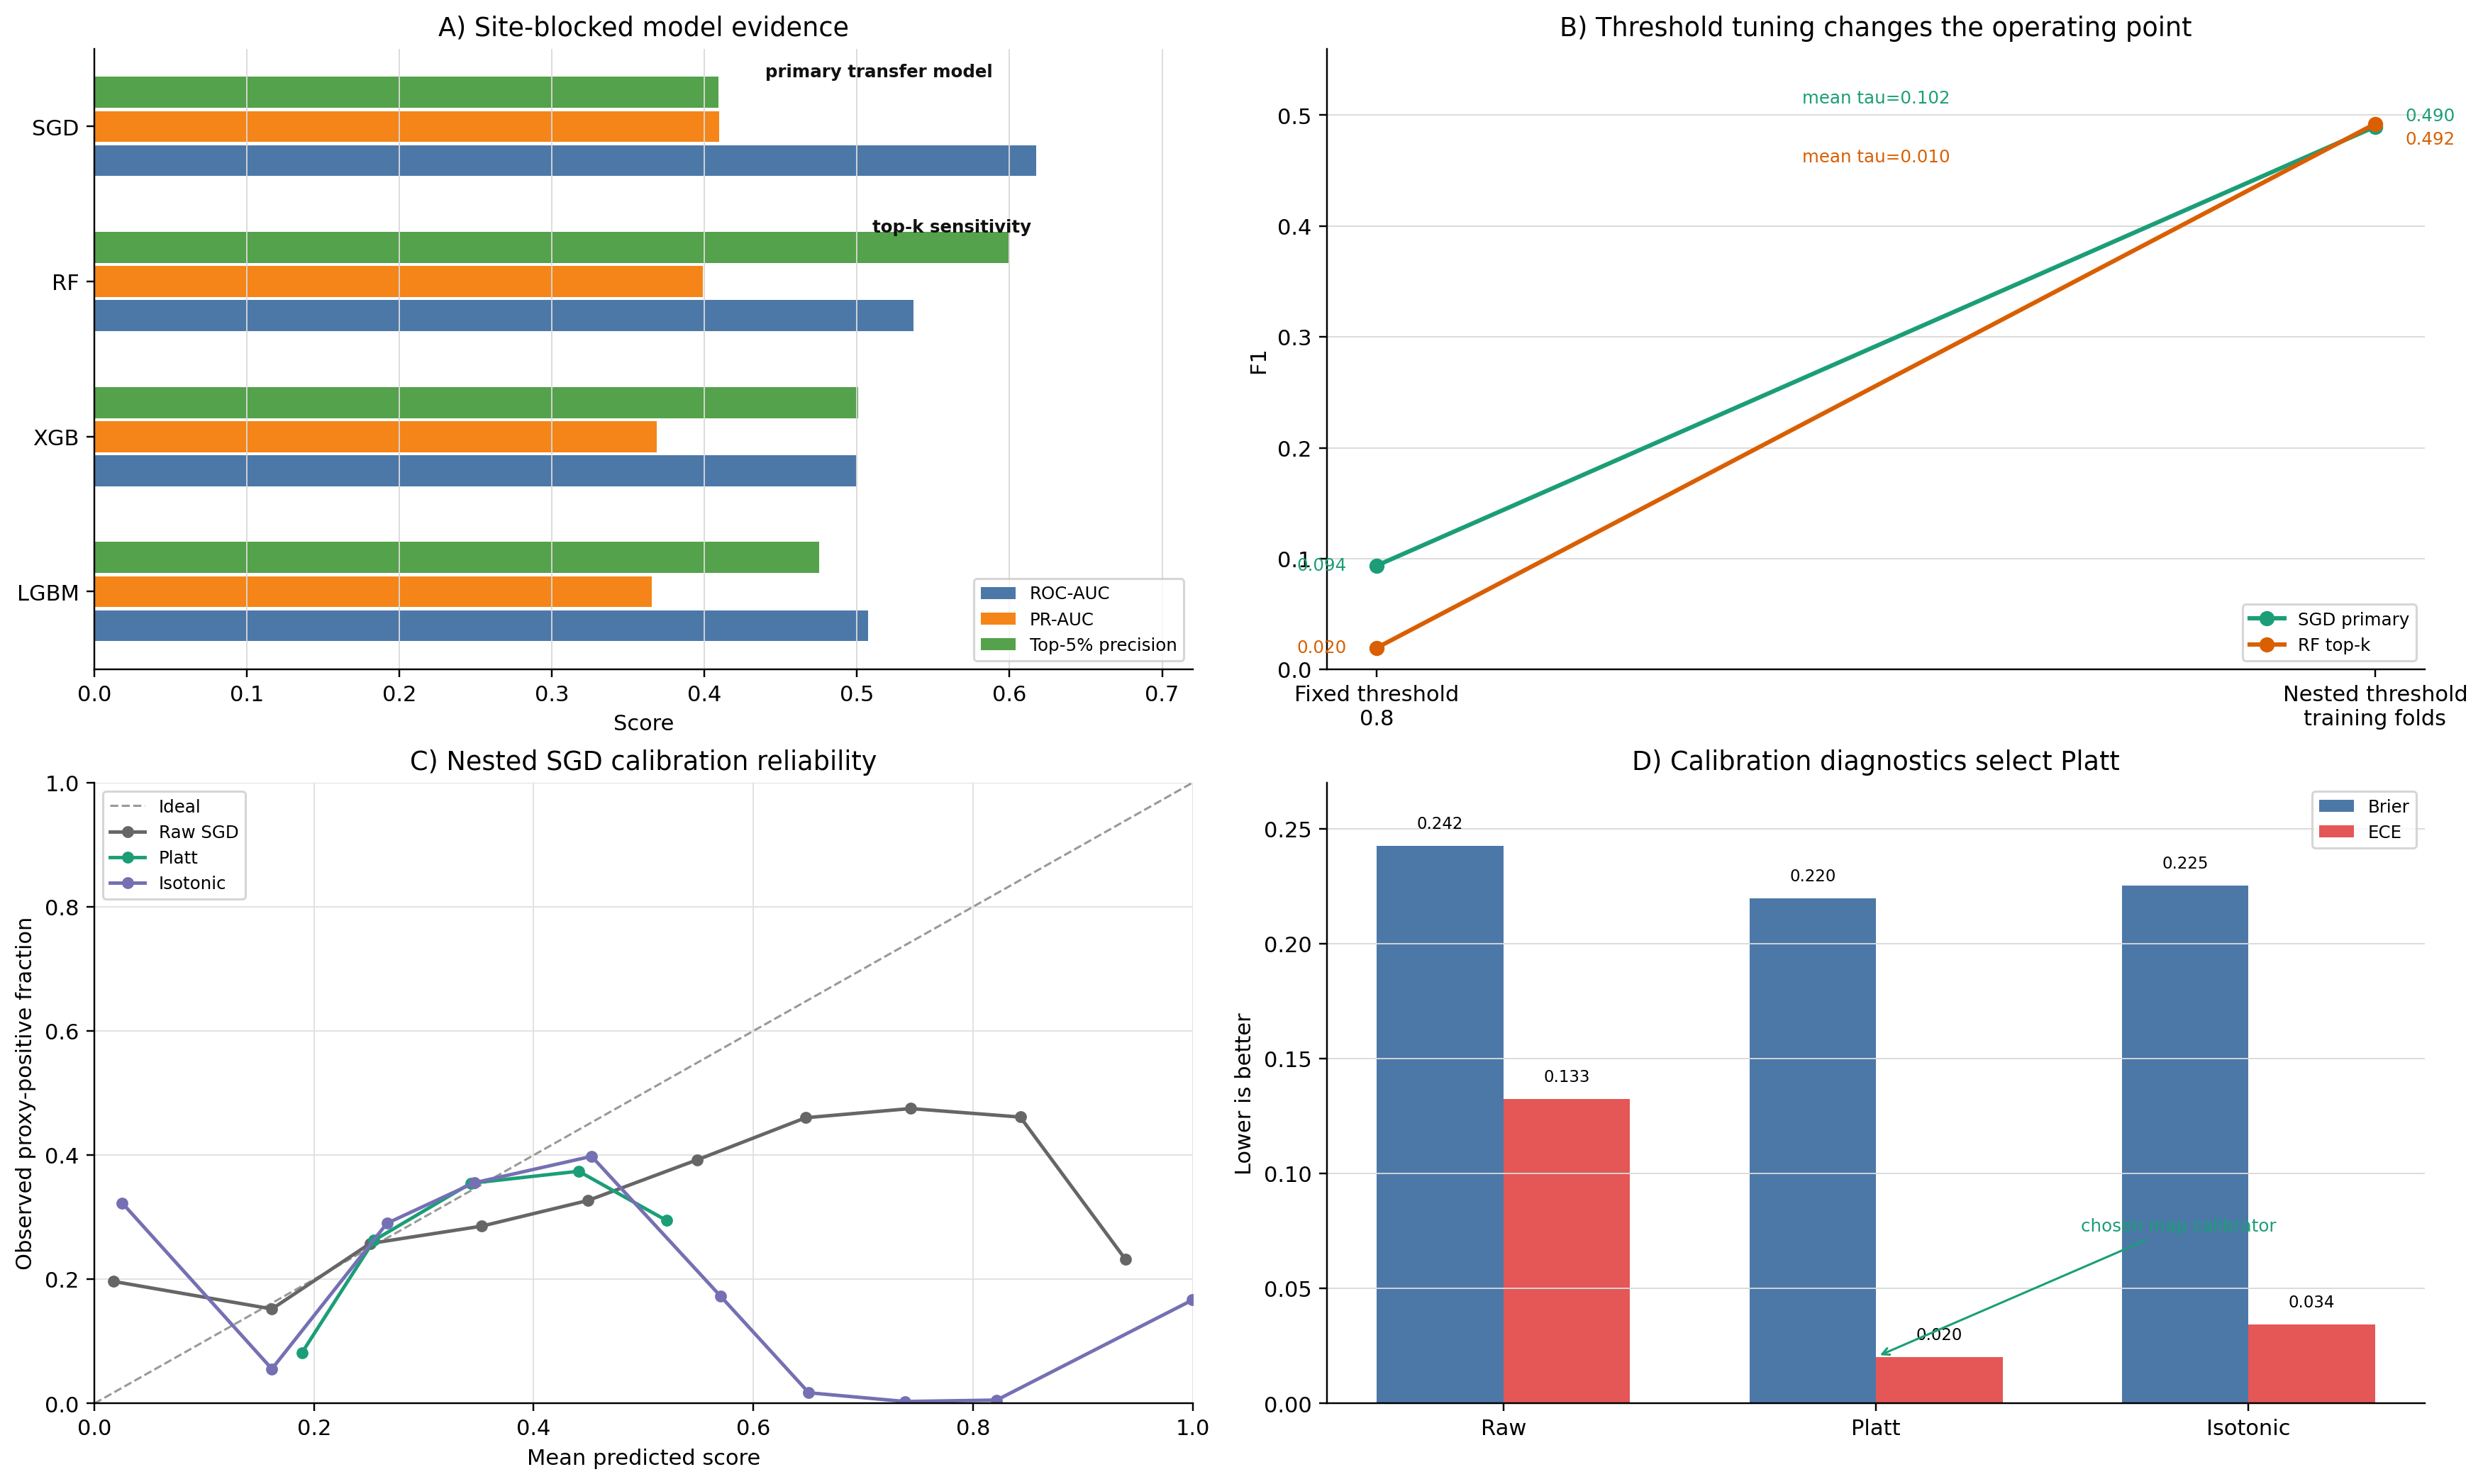
\includegraphics[width=\textwidth]{figures/03_validation/fig03_validation_summary.png}
\caption{Validation summary for model selection. Panel A compares site-blocked ranking metrics, Panel B shows nested threshold effects on F1, Panel C gives SGD calibration reliability, and Panel D reports Brier score and expected calibration error.}
\label{fig:validation-summary}
\end{figure}

The result is instructive. The tree models can find strong within-region partitions, but those partitions appear partly site-specific. The SGD model has less expressive power, and that constraint seems to help it preserve the broader cross-site signal. We therefore use SGD as the primary spatial-transfer model. Random forest is not discarded; it is retained as a sensitivity model because it concentrates true proxy positives well in the top-ranked fraction. Its role, however, is ranking stress-test rather than calibrated probability mapping.

\subsection{Hyperparameter tuning confirmed the model choice}
Focused site-blocked tuning did not overturn the initial selection. The best SGD trial used \(\alpha=10^{-4}\) and obtained the same pooled ROC-AUC 0.6173 and PR-AUC 0.4096 as the comparison run. Nearby SGD alphas produced similar but slightly weaker PR-AUC values. The best RF trial used 400 trees with unrestricted depth and reached PR-AUC 0.3995 with top-5\% precision 0.6038. Tuned XGBoost and LightGBM trials remained below SGD under the site-blocked criterion.

This matters because it reduces the chance that the SGD result is an accident of an untuned baseline. The current evidence says that, for these proxy AOIs and this feature stack, the strongest transferable signal is captured by a simple regularized classifier. A more complex model may still be useful for generating alternative rankings, but it should not be promoted to the main scientific model unless it wins under the same site-blocked rule.

\subsection{Threshold tuning rescued F1, but also exposed prevalence sensitivity}
The legacy fixed threshold of 0.8 was too conservative for the sampled validation distribution. Nested threshold tuning improved SGD F1 from 0.0937 to 0.4896, with a mean selected threshold of 0.102. RF F1 similarly improved from 0.0196 to 0.4922, but all RF outer folds selected the minimum tested threshold of 0.01. Table~\ref{tab:threshold-calibration} shows the main threshold and calibration results.

\begin{table}[t]
\centering
\caption{Nested threshold tuning and SGD calibration. Thresholds are selected inside training folds, and calibration metrics are pooled site-blocked diagnostics for SGD.}
\label{tab:threshold-calibration}
\begin{tabular}{llrrrr}
\toprule
Analysis & Model or calibrator & Main metric & Precision & Recall & F1 or ECE \\
\midrule
Fixed threshold & SGD, \(\tau=0.8\) & PR-AUC 0.4096 & 0.3984 & 0.0531 & F1 0.0937 \\
Nested threshold & SGD, mean \(\tau=0.102\) & PR-AUC 0.4096 & 0.3389 & 0.8822 & F1 0.4896 \\
Nested threshold & RF, \(\tau=0.01\) & PR-AUC 0.3995 & 0.3347 & 0.9298 & F1 0.4922 \\
Calibration & Raw SGD & Brier 0.2425 & -- & -- & ECE 0.1325 \\
Calibration & Platt SGD & Brier 0.2197 & -- & -- & ECE 0.0202 \\
\bottomrule
\end{tabular}
\end{table}

The tuned thresholds should not be read as universal map cutoffs. They are valid for fold-level evaluation because they were selected without looking at the held-out site, but they reflect the controlled validation prevalence: each site sample contains one positive pixel for approximately two background pixels. The natural landscape prevalence of hydrogen-favorable conditions is almost certainly lower. Thus, thresholded F1 is useful for comparing models under the sampled experiment, while prospectivity maps should be read as ranked and calibrated screening surfaces.

\subsection{Platt calibration made the SGD score usable for cautious mapping}
Raw SGD scores ranked best, but their probability scale was poorly calibrated. Platt calibration reduced Brier score from 0.2425 to 0.2197 and reduced 10-bin expected calibration error from 0.1325 to 0.0202. Isotonic calibration also improved calibration relative to raw SGD, but it was less stable across sites and had weaker pooled ranking diagnostics. We therefore use the raw SGD scores for ROC-AUC and PR-AUC interpretation, while using Platt-calibrated SGD for the final prospectivity-score raster.

This distinction is subtle but important. Calibration does not create field truth. It only makes the model score more consistent with the sampled proxy-label distribution. The final raster is therefore named and interpreted as a calibrated prospectivity score, not as a probability that a pixel contains natural hydrogen.

\subsection{Final prospectivity maps and site-level review}
The final map generation fitted SGD, a Platt calibrator, and the RF sensitivity model using all strict-valid site samples, then streamed the full feature stack by raster windows. The SGD Platt raster has mean score 0.3208 over strict-valid pixels, with Q95 0.4546 and Q99 0.5098. RF top-k sensitivity thresholds were 0.8975 for the top 1\%, 0.5125 for the top 5\%, and 0.3350 for the top 10\%. Because RF scores are discrete in many places, top-k mask counts can slightly exceed the nominal fraction when many pixels share the threshold score.

Table~\ref{tab:final-raster-summary} records the final raster statistics used to interpret these surfaces. The important pattern is that the calibrated SGD score has a compressed range rather than a dramatic high-probability tail. That is appropriate for a proxy-label screening study: the map is ranking plausible follow-up zones, not certifying occurrence.

\begin{table}[t]
\centering
\caption{Final raster product statistics over strict-valid pixels. RF thresholds define rank-based sensitivity zones, and SGD values define Platt-calibrated prospectivity scores for the sampled proxy-label distribution.}
\label{tab:final-raster-summary}
\begin{tabular}{llr}
\toprule
Product & Statistic & Value \\
\midrule
Strict valid-data mask & Valid pixels scored & 21,971,235 \\
SGD Platt prospectivity score & Mean & 0.3208 \\
SGD Platt prospectivity score & Q95 & 0.4546 \\
SGD Platt prospectivity score & Q99 & 0.5098 \\
RF sensitivity score & Top-1\% threshold & 0.8975 \\
RF sensitivity score & Top-5\% threshold & 0.5125 \\
RF sensitivity score & Top-10\% threshold & 0.3350 \\
\bottomrule
\end{tabular}
\end{table}

The site-level review figure makes the same point spatially. Figure~\ref{fig:final-site-review} shows four panels for each site: the SGD Platt prospectivity score, the continuous RF ranking score, the RF top-5\% sensitivity zone, and strict valid-data coverage. This pairing is deliberate. The SGD panel gives the primary calibrated screening surface. The RF score panel then asks whether a nonlinear ranker organizes the same local neighborhoods into similar high-ranking structure, while the binary RF top-5\% panel makes that ranking test spatially explicit. The coverage panel closes the loop by preventing interpretation where the feature stack is incomplete.

\begin{sidewaysfigure}[p]
\centering
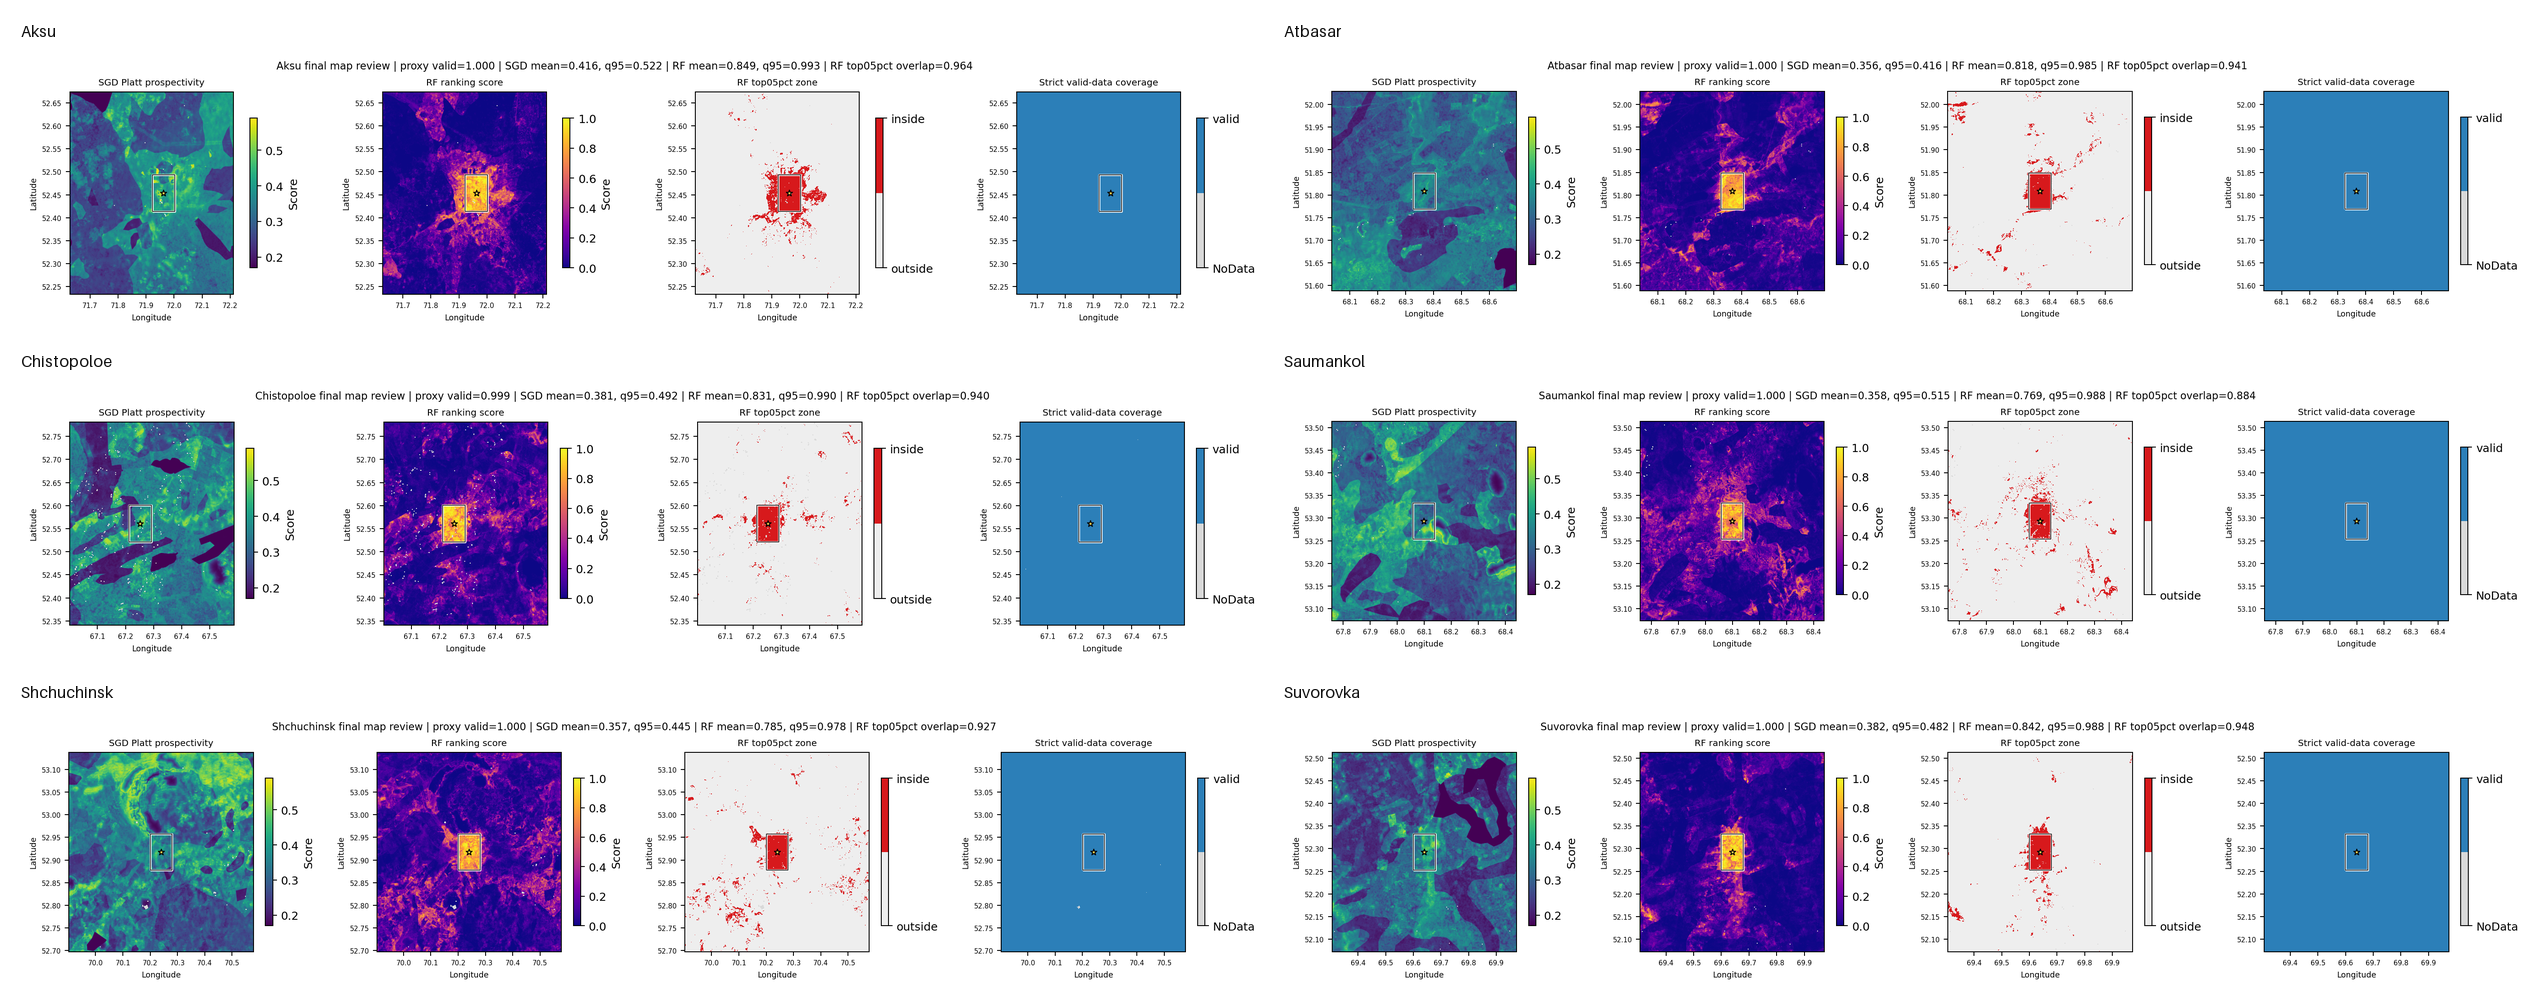
\includegraphics[width=0.94\textheight,height=0.80\textwidth,keepaspectratio]{figures/04_final_maps/final_site_figures_contact_sheet.png}
\caption{Final site-level review panels for the six proxy AOIs. Panels show SGD Platt prospectivity, RF ranking score, RF top-5\% sensitivity zone, and strict valid-data coverage. RF products are ranking diagnostics, not calibrated probabilities.}
\label{fig:final-site-review}
\end{sidewaysfigure}

All six proxy AOIs have near-complete strict-valid coverage (Table~\ref{tab:site-review-summary}); Chistopoloe is the lowest at 0.999. Mean SGD Platt scores inside the proxy AOIs range from 0.356 at Atbasar to 0.416 at Aksu. RF ranking-score means range from 0.769 at Saumankol to 0.849 at Aksu, and RF top-5\% overlap inside proxy AOIs ranges from 0.884 at Saumankol to 0.964 at Aksu. This agreement is useful as an internal consistency check, but it is still model agreement against proxy AOIs rather than an independent hydrogen confirmation.

\begin{table}[t]
\centering
\caption{Site-level final-map diagnostics inside proxy AOIs. SGD values are Platt-calibrated prospectivity scores. RF mean, RF Q95, and RF overlap are internal ranking diagnostics rather than independent validation.}
\label{tab:site-review-summary}
\begin{tabular}{lrrrrrr}
\toprule
Site & \shortstack{Strict-valid\\fraction} & \shortstack{SGD\\mean} & \shortstack{SGD\\Q95} & \shortstack{RF\\mean} & \shortstack{RF\\Q95} & \shortstack{RF top-5\%\\overlap} \\
\midrule
Aksu & 1.000 & 0.416 & 0.522 & 0.849 & 0.993 & 0.964 \\
Atbasar & 1.000 & 0.356 & 0.416 & 0.818 & 0.985 & 0.941 \\
Chistopoloe & 0.999 & 0.381 & 0.492 & 0.831 & 0.990 & 0.940 \\
Saumankol & 1.000 & 0.358 & 0.515 & 0.769 & 0.988 & 0.884 \\
Shchuchinsk & 1.000 & 0.357 & 0.445 & 0.785 & 0.978 & 0.927 \\
Suvorovka & 1.000 & 0.382 & 0.482 & 0.842 & 0.988 & 0.948 \\
\bottomrule
\end{tabular}
\end{table}

These overlaps are encouraging as an internal QA result because the final rasters recover the proxy AOIs after strict NoData masking and independent-prior integration. They are not independent confirmation. The proxy AOIs helped define the training labels, so strong overlap means the carried-forward models preserve the supervised signal around reported sites while still requiring field deployment before any detection claim can be made.

\section{Discussion}
The main contribution of this experiment is not the production of a visually persuasive prospectivity map. It is the construction of an evidence hierarchy that makes the map harder to overread. Natural hydrogen exploration is attractive precisely because the potential source systems are broad: serpentinization, radiolysis, deep crustal degassing, water-rock reaction, and migration through structural pathways can all produce surface or near-surface expressions \cite{zgonnik2020occurrence}. That breadth also makes remote prediction dangerous. A spectral anomaly, lineament, lithologic class, or terrain break is rarely diagnostic by itself. In this study, those layers are treated as weak, indirect evidence. The map asks where the combined evidence resembles the proxy anomaly neighborhoods under a leakage-aware validation rule; it does not ask the satellite record to replace field gas measurement.

The strict NoData decision is therefore central to the scientific interpretation. Filling missing Sentinel-2, Landsat-8, lithology, or fault-prior values with synthetic substitutes would have produced a more complete raster, but the resulting map would have mixed observation with invention. For a screening workflow, that distinction matters more than cartographic completeness. The SRTM, Sentinel-2, Landsat-8, GLiM, and GEM sources are all defensible published products \cite{farr2007srtm,drusch2012sentinel,roy2014landsat8,hartmann2012glim,styron2020gem}, but their uncertainty structures are not interchangeable. The coverage audit made those structures visible before the model was interpreted. Once the positive AOIs passed the strict-valid gate, the dominant question shifted from ``do we have enough pixels?'' to ``does the learned relationship transfer when an entire site is withheld?''

That second question explains why the simpler SGD model became the primary study model. In ordinary random pixel splits, flexible tree ensembles can appear superior because neighboring pixels share acquisition conditions, geomorphology, land cover, and label geometry. Site-blocked validation removes that comfort. It asks the model to generalize from five reported sites to a sixth, which is closer to the actual field problem. The result is consistent with the broader spatial-validation literature: when spatial dependence is strong, random folds can be optimistic, and blocked folds are a better test of transfer \cite{roberts2017crossvalidation,valavi2019blockcv}. The regularized SGD classifier had less capacity to memorize local texture, and that constraint appears to have helped it retain the broadest cross-site signal.

\begin{sidewaystable}[p]
\centering
\small
\caption{Model-source and hyperparameter comparison for the screening experiment. The table reports algorithm sources, screening rationale, tuned hyperparameters, and study roles after strict site-blocked validation.}
\label{tab:model-source-hyperparameters}
\begin{tabular}{p{0.16\textwidth}p{0.18\textwidth}p{0.26\textwidth}p{0.22\textwidth}p{0.18\textwidth}}
\toprule
Model family & Algorithm or implementation source & Screening rationale & Hyperparameters in this study & Outcome and study role \\
\midrule
Regularized SGD logistic classifier & scikit-learn SGD implementation \cite{pedregosa2011scikit} & Low-capacity linear baseline for transferable signal across sites; suitable when proxy labels are sparse and spatially clustered. & StandardScaler; loss = log loss; class weight = balanced; \(\alpha\in\{10^{-5},3\times10^{-5},10^{-4},3\times10^{-4},10^{-3}\}\); selected \(\alpha=10^{-4}\); max\_iter = 4000. & Best pooled site-blocked ROC-AUC and PR-AUC (0.6173 and 0.4096). Carried forward as the primary Platt-calibrated prospectivity raster. \\
Random forest & Breiman random forest ensemble \cite{breiman2001randomforests} & Nonlinear benchmark for mixed terrain, spectral, lithology, and structural predictors; useful for top-ranked sensitivity zones. & class\_weight = balanced\_subsample; n\_estimators \(\in\{200,400\}\); max\_depth \(\in\{8,\mathrm{None}\}\); selected n\_estimators = 400 and max\_depth = None. & Weaker primary PR-AUC than SGD, but best top-5\% precision after tuning (0.6038). Retained as RF ranking-score and top-k sensitivity product, not as a calibrated probability map. \\
XGBoost & Scalable gradient tree boosting \cite{chen2016xgboost} & High-capacity nonlinear model for interactions among spectral response, terrain, lithology, and lineament priors. & n\_estimators = 120; max\_depth \(\in\{3,5\}\); learning\_rate \(\in\{0.05,0.1\}\); scale\_pos\_weight set from training-fold class balance. & Strong diagnostic benchmark under conventional expectations, but weaker than SGD under strict site-blocked transfer. Not carried into final map products. \\
LightGBM & Histogram-based gradient boosting \cite{ke2017lightgbm} & Efficient boosted-tree alternative to test whether leaf-wise boosting improves spatial transfer. & n\_estimators = 200; num\_leaves \(\in\{15,31\}\); learning\_rate \(\in\{0.05,0.1\}\); class\_weight = balanced. & Did not outperform SGD or RF under the site-blocked criterion. Retained only as a benchmark in the validation evidence. \\
\bottomrule
\end{tabular}
\end{sidewaystable}

The comparison in Table~\ref{tab:model-source-hyperparameters} also clarifies why RF is retained rather than discarded. RF did not provide the best transferable calibrated surface, but it concentrated many proxy-positive pixels in the most aggressive top-ranked fraction. That makes it valuable as a sensitivity model. In practice, the SGD and RF outputs answer different questions. The SGD Platt map asks for the most stable calibrated prospectivity surface under the sampled proxy-label distribution. The RF ranking map asks whether a more nonlinear model points to similar zones when allowed to emphasize sharper feature interactions. Agreement between the two is encouraging; disagreement is informative because it highlights places where model form, rather than data coverage alone, controls the ranking.

The calibration result should also be read narrowly. Platt calibration improved the SGD score scale, but it did not convert a proxy label into an independent hydrogen observation \cite{platt1999probabilistic}. The calibrated value is tied to the training sample design, where each site contributes a controlled ratio of positive proxy pixels to local-background pixels. The natural prevalence of hydrogen-favorable conditions across northern Kazakhstan is not known and is almost certainly lower than the sampled prevalence. For the same reason, nested threshold tuning is useful for comparing models but not for defining a universal exploration cutoff. Precision-recall diagnostics are appropriate because the intended detection class is sparse \cite{saito2015precision}, yet even improved F1 should be interpreted as sampled-fold behavior, not regional occurrence probability.

The external-prior result is scientifically useful even though it is modest. GLiM lithology added regional geological context, and the model used several lithology classes. However, GLiM is global and coarse relative to a field prospect. It can separate broad rock-type settings but cannot resolve alteration, fracture permeability, soil-gas pathways, groundwater chemistry, or site-scale stratigraphy. The GEM active-fault result is similarly instructive. No active-fault traces were returned inside the buffered AOI, so the fault distance and density bands carried little signal. That absence should not be interpreted as proof that faults are absent. It means only that the selected public active-fault source did not map active traces in the modeled window. A more detailed Kazakhstan structural inventory could change the fault-prior layer without contradicting the DEM or optical stack.

The site-level final maps should therefore be used as field-planning aids. Aksu has the highest proxy-AOI SGD mean and RF mean in the current final figures, while Saumankol has high SGD Q95 but the lowest RF top-5\% overlap among the six sites. Those differences are not a ranking of proven hydrogen resources. They are an ordered set of hypotheses about where follow-up sampling may be most efficient. The most defensible deployment plan would combine the map with field measurements that the current workflow does not contain: soil-gas hydrogen concentration, flux repeatability, gas composition, isotope constraints, lithologic logging, fracture mapping, and seasonal repeat surveys. Those measurements should then replace proxy labels in a future supervised run.

This framing also guides whether more complex models, including quantum machine-learning variants, should be added. Additional models are useful only if they are judged under the same blocked validation, strict NoData masking, and calibration rules. A model that improves random-split accuracy but fails leave-one-site-out transfer would make the study more crowded without improving the science. Conversely, a new model that beats the SGD primary model under the same spatial gate, or that exposes complementary uncertainty in a clearly labeled sensitivity product, would be worth reporting. Until then, the current evidence supports a conservative hierarchy: SGD for the main calibrated screening surface, RF for nonlinear ranking sensitivity, and XGBoost/LightGBM as documented benchmarks.

The broader implication is that early natural-hydrogen screening should be designed as a reproducible triage system rather than as a discovery claim. The workflow is strongest where it refuses easy shortcuts: it preserves NoData, separates sites during validation, distinguishes calibration from truth, and names RF zones as rank diagnostics. These constraints make the result less dramatic, but more useful. A field team can inspect why a site was prioritized, see where the input stack is valid, and understand which model family supports the ranking. That is the right level of confidence for a proxy-supervised study. The next scientific step is not to make the current map more certain by narration; it is to collect independent measurements that can test, correct, and eventually replace the proxy target.

\section{Current limitations}
Three limitations control the strength of the claims. First, the labels are proxy polygons around reported anomaly coordinates rather than field-confirmed hydrogen measurements. Second, the strongest validation design available here is leave-one-site-out across six sites, which is much better than random pixel splitting but still a small spatial sample. Third, the final calibrated scores are tied to a controlled sample prevalence and should not be interpreted as natural prevalence in the landscape. These limitations do not invalidate the workflow. They define its proper use: reproducible prioritization for field follow-up, with uncertainty and proxy-label caveats carried forward into the figures and captions.

\section{Conclusion}
This study establishes a leakage-aware workflow for natural hydrogen prospectivity screening in northern Kazakhstan using multisource terrain, optical, lithology, and structural-prior evidence. The central result is methodological as much as predictive: when strict NoData handling and leave-one-site-out validation are enforced, the strongest transferable signal is captured by a regularized SGD logistic model rather than by higher-capacity tree ensembles. This outcome supports a cautious screening hierarchy. The Platt-calibrated SGD raster provides the primary prospectivity surface for field prioritization, while the random-forest ranking score and top-k zones provide nonlinear sensitivity evidence. XGBoost and LightGBM remain useful benchmarks, but they do not justify replacement of the primary model under the spatial-transfer criterion used here.

The study also shows that data provenance controls interpretation. Rebuilt Sentinel-2 and Landsat-8 composites remove the earlier positive-AOI coverage blocker, GLiM lithology adds independent regional geological context, and the GEM active-fault query documents the absence of mapped active-fault traces in the selected public source. None of these layers directly detects hydrogen. Their value lies in reproducibly organizing indirect evidence around reported anomaly sites while preserving the difference between observation, proxy supervision, and field confirmation. This provides a clear audit trail for later comparison when field measurements become available and the proxy targets can be challenged directly in practice.

The resulting maps should therefore be used as planning tools for targeted deployment rather than as discovery products. High-ranked zones identify locations where soil-gas surveys, repeated flux measurements, gas composition analysis, isotope work, field structural mapping, and local lithologic verification can be concentrated efficiently. The next scientific step is to replace proxy AOI labels with measured hydrogen observations and rerun the same blocked validation design. If future field data confirm that the mapped rankings predict independent hydrogen measurements, the workflow can mature from proxy-screening into a robust field-tested regional exploration model.

\bibliographystyle{plainnat}
\bibliography{ex_01}

\end{document}
